\documentclass[11pt]{article}

% --- arXiv-friendly, journal-agnostic single-column setup ---
\usepackage[utf8]{inputenc}
\usepackage[T1]{fontenc}
\usepackage{lmodern}
\usepackage[margin=1in]{geometry}
\usepackage{amsmath,amssymb,amsthm}
\usepackage{algorithm}
\usepackage{algpseudocode}
\newtheorem{proposition}{Proposition}
\newtheorem{assumption}{Assumption}
\usepackage{graphicx}
\usepackage{booktabs}
\usepackage{natbib}
\setlength{\bibsep}{0.3ex plus 0.2ex}
\usepackage{multicol}
\usepackage{lineno}
\usepackage{hyperref}
\hypersetup{colorlinks=true,linkcolor=blue,citecolor=blue,urlcolor=blue}
% Allow long URLs/DOIs to break at punctuation (needed for two-column references)
\makeatletter
\g@addto@macro\UrlBreaks{\do\/\do\-\do\.\do\=\do\?\do\&\do\_\do\:}
\makeatother
\Urlmuskip=0mu plus 1mu\relax
% Float-packing: allow more float area per page in this float-heavy paper
\renewcommand{\topfraction}{0.92}
\renewcommand{\bottomfraction}{0.85}
\renewcommand{\textfraction}{0.08}
\renewcommand{\floatpagefraction}{0.75}
\setcounter{topnumber}{3}
\setcounter{totalnumber}{5}

\title{Uncertainty-Aware Fire Risk Assessment for UK Residential Buildings
Using Public Data and Mechanism-Informed Simulation}

\author{Matthew Reid}
\date{\today}

\begin{document}
\linenumbers
\maketitle

\begin{abstract}
Fire risk assessment in the UK built environment remains largely periodic,
qualitative, and compliance-oriented, despite the availability of public
incident, building, demographic, and regulatory data. This paper develops an
uncertainty-aware framework for residential fire-risk assessment and targeting
in England. We combine public fire incident statistics, Energy Performance
Certificate records, deprivation indices, Census occupancy proxies, care-home
registers, and fire-service geography into an open, validated,
UPRN-keyed (dwelling-level) database, and estimate calibrated posterior distributions for
dwelling-fire occurrence and consequence-relevant outcomes. A hierarchical
negative-binomial model predicts annual small-area dwelling-fire counts with
held-out probabilistic calibration; record-level consequence models estimate
serious spread and casualty associations under explicit treatment of
alarm-state confounding, separating predictive association from intervention
effect. To represent building mechanisms not observed in public registers, we
introduce a transparent, mechanism-informed archetype fire/egress simulator,
benchmark it against observed spread and casualty margins and a documented
real-building boundary case, and compress its outputs into interpretable
consequence surrogates. We then demonstrate decision-theoretic prevention
targeting: under stated assumptions, a fixed smoke-alarm visit budget averts
substantially more harm when allocated by posterior risk and expected benefit
than by random or deprivation-only rules. The paper contributes a calibrated,
auditable public-data decision framework for fire-risk prioritisation, and
sets out a latent-state extension in which inspection findings are treated as
noisy observations for live risk updating --- providing a first partial
instantiation on 1{,}441 published fire risk assessments: a fitted
measurement model, a worked single-building posterior update, and first
empirical bounds on assessor detection sensitivity, with full structural
identification awaiting repeated assessment waves.
\end{abstract}

\section{Introduction}
\label{sec:intro}

Fire in the UK residential built environment remains a large and, recently, a
growing problem: fire and rescue services attended 40{,}350 building fires in
England in the year ending December 2025, up 5.5\% year-on-year, of which 26{,}298
were dwelling fires \citep{mhclg2026firestats}. Yet the fire risk assessment (FRA)
that governs those buildings is still periodic, qualitative, and compliance-driven
--- checklist judgements recorded under the Regulatory Reform (Fire Safety)
Order \citep{rrfso2005} and codified methodologies such as PAS~79
\citep{pas79_1_2020,pas79_2_2020}. The Grenfell Tower fire and the Phase~2 Inquiry
reframed residential fire safety around evidence, accountability, and the active
management of higher-risk buildings \citep{grenfell2024phase2}, and the regulatory
response --- the Fire Safety Act 2021 \citep{firesafetyact2021} and the Building
Safety Act 2022 \citep{bsa2022}, with their safety-case regime --- demands exactly
the kind of quantitative, evidence-updated risk picture that current practice does
not produce.

Three gaps stand out. Risk is communicated as a categorical score rather than a
distribution, despite evidence that risk matrices have poor resolution and can rank
worse than random \citep{cox2008,thomas2014}. Inspection findings are treated as
ground truth rather than as noisy, intermittent observations; a targeted search
across the fire-risk-assessment, inter-rater-reliability, assessor-variability, and
PAS~79 literatures surfaced competence standards and professional guidance, but we
are not aware of any empirical study estimating inter-assessor variability from
repeated assessments of the same UK residential building --- the sector's response
has been a competence standard \citep{bs8674_2025} rather than measurement
of assessor noise --- motivating the noisy-observation treatment we import from
structural risk-based inspection \citep{straub2005,luque2019}. And fire outcomes are
rare events, yet calibration and uncertainty quantification (UQ) are seldom made
explicit in operational FRA, even as reviews of fire machine learning confirm that
UQ and calibration remain underdeveloped \citep{tapehnaser2022} against an established
calibration-and-sharpness standard \citep{gneiting2007}.

We recast FRA as Bayesian inference under uncertainty: a building's fire risk is a
posterior distribution over ignition, spread, evacuation failure, and consequence
severity, inferred from heterogeneous public evidence and updateable as new
observations arrive. The novelty is not a new Bayesian network, a new fire
simulator, or a new evacuation model in isolation; it is an auditable decision
framework that couples calibrated UK open-data rare-event modelling,
mechanistically grounded consequence simulation, uncertainty propagation, and
decision-theoretic prevention targeting into one posterior-risk workflow. The paper
is explicit throughout about what is built and what is specified: the calibrated
public-data and simulation components below are \emph{implemented}, while the
latent-state, noisy-inspection extension for live risk updating
(Section~\ref{sec:model}) is \emph{proposed} --- fully specified but not yet fully
instantiated. Five contributions follow:

\begin{enumerate}
  \item A UK open-data fire-risk database linking incident, building-stock,
        deprivation, occupancy, and vulnerability evidence at dwelling and
        small-area scale, validated against published totals
        (Section~\ref{sec:data}).
  \item A calibrated rare-event occurrence model for dwelling fires ---
        hierarchical negative-binomial with out-of-time probabilistic validation
        (Section~\ref{sec:results}).
  \item Consequence models that explicitly separate predictive association from
        intervention effect, with formal treatment of alarm-state confounding,
        alongside a mechanism-informed archetype fire/evacuation simulator that
        supplies consequence estimates where public geometry and evacuation data
        do not exist (Section~\ref{sec:surrogate}).
  \item A decision-theoretic targeting demonstration: under stated assumptions, a
        fixed prevention budget allocated by posterior risk and expected benefit
        returns roughly nine times the value of untargeted allocation and 2.5
        times deprivation-only targeting (Section~\ref{sec:results-decision}).
  \item A proposed latent-state formulation in which inspection findings enter as
        noisy observations (Section~\ref{sec:model}), motivated by the
        measurement-error tradition of structural risk-based inspection, together
        with a real-building stress test bounding the simulator's regime
        assumptions against Grenfell Tower
        (Section~\ref{sec:results-casestudy}).
\end{enumerate}

\section{Related Work}
\label{sec:related}

We organise prior work along the eight themes that emerged from a systematic
sweep of the literature, and position our integration against each. Seven
differentiators recur: (A) UK FRA / Building-Safety-Act integration; (B)
Bayesian latent-state inference of building condition; (C) calibrated
uncertainty with missing-evidence flags; (D) inspection as noisy observation;
(E) rare-event outcome treatment; (F) a mechanism-informed consequence
surrogate; and (G) decision-theoretic inspection prioritisation.

\paragraph{UK fire-safety landscape and FRA methodology.}
A recent systematic review of UK building fire-safety practice catalogues its
technological, mitigation, behavioural, and regulatory strands, and flags
persistent compliance, enforcement, and maintenance gaps \citep{dauda2025uk};
the Hackitt review diagnosed a ``broken'' regulatory system and seeded the
outcomes-based safety-case regime that followed \citep{hackitt2018,perry2025}.
Quantitative fire risk assessment itself has a long lineage --- event-tree and
deterministic consequence analysis in textbook form \citep{yung2008,rasbash2004},
statistics-driven residential risk indices \citep{xin2013}, single-factor
effectiveness estimates such as smoke-alarm impact \citep{gilbert2021}, and
UK-specific trend analyses of accidental dwelling fires \citep{taylor2026}.
This literature motivates our setting (A) but is either policy diagnosis or
static, deterministic assessment; what an ``evidence-based'' regime lacks, and
what we supply, is the probabilistic latent-state machinery (B, C).

\paragraph{Probabilistic and Bayesian-network fire-risk models.}
The closest prior line chains fire development, escape, and intervention for UK
dwellings in three-part Bayesian networks (BNs)
\citep{matellini2018threepart,matellini2013}, alongside BN fatality and spread
models \citep{hanea2009,cheng2009} and a credal-network probabilistic risk
assessment of fire occurrence applied to Grenfell Tower
\citep{estradalugo2019grenfell}. More recent variants extend the construction
to heritage buildings \citep{chen2023hist}, subway and tunnel scenario
evolution \citep{li2024subway,hidayat2025tunnel}, and high-rise electrical and
fuzzy composite scoring \citep{su2023electrical,wang2021fuzzy,tan2021tho}, all
on the BN foundations of \citet{pearl1988}. We adopt this tradition's
latent-state, posterior view of risk --- but throughout it, conditional
probability tables (CPTs) are fixed from expert judgement or aggregate
statistics, inputs are treated as certain, and outputs are points: no
calibrated uncertainty (C), no treatment of inspections as noisy observations
(D), no physics-based consequence layer (F), and no inspection-prioritisation
layer (G).

\paragraph{Uncertainty quantification and decision-theoretic inspection.}
Risk matrices --- the format operational FRA actually uses --- have poor
resolution and can rank risks worse than random \citep{cox2008,thomas2014},
while calibration and sharpness under proper scoring rules provide the
evaluation standard for probabilistic forecasts that we adopt
\citep{gneiting2007}. Separately, the structural-reliability
risk-based-inspection and value-of-information tradition treats inspections as
imperfect information that updates a reliability estimate, and optimises
inspection planning on that basis
\citep{straub2005,luque2019,zhang2021voi,vereecken2020,klerk2019}. Our
contribution here is a transplant: importing inspection-as-noisy-observation
(D) and expected value of inspection (G) into fire risk assessment, and
replacing categorical scores with posterior distributions (C) --- a combination
this tradition has never instantiated for fire.

\paragraph{Fire-risk datasets, geospatial mapping, and service targeting.}
England-wide small-area evidence links deprivation to fire-related dwelling
casualties \citep{li2022}; emergency-service demand analytics
\citep{londonblue2025} and evaluations of home-fire-safety-visit targeting
\citep{waring2024} supply the operational context, with hierarchical Bayesian
small-area rate estimation as the methodological template \citep{macnab2003}.
The open-datacube precedent is IberFire, a spatio-temporal wildfire-risk cube
assembled entirely from open sources \citep{erzibengoa2025iberfire}. These
works supply our covariates and the open-data blueprint (A), but remain
ecological and associational: none couples the data to a building-conditioned
probabilistic model with quantified uncertainty (B, C).

\paragraph{Machine learning in fire safety.}
Reviews of fire-safety machine learning map a fast-growing field and flag
precisely the weaknesses we target: underdeveloped uncertainty quantification
and calibration \citep{yildiz2025ml,tapehnaser2022}, with mechanistically grounded
learning advocated as the remedy \citep{naser2021}. Applications span
smart-building design \citep{zeng2024smart}, classifiers explained post hoc
with SHapley additive explanations (SHAP) \citep{lu2023stadium,dai2025interp},
and knowledge-graph and city-scale forecasting
\citep{xu2025knowgraph,lee2025urbanfire}. We use machine learning differently:
as a calibrated surrogate \emph{inside} a probabilistic model (C, F), rather
than as a black-box or post-hoc-explained point classifier.

\paragraph{Fast fire-simulation surrogates.}
A systematic review of physics-informed surrogates finds them rarely embedded
inside a probabilistic risk model \citep{yarmohammadian2025pism} --- the
integration gap this paper occupies. The component technology is mature:
emulators predict fire fields, flashover, and detection orders of magnitude
faster than computational fluid dynamics
\citep{lattimer2020,wang2021pflash,nguyen2022,zeng2022ifetool,zeng2024jcde};
physics-informed neural networks learn interpretable spread parameters
\citep{vogiatzoglou2025}; probabilistic diffusion surrogates output spread
ensembles \citep{yu2026}; and graph neural networks serve as surrogates over
building-block graphs \citep{wu2025gnn}. We adopt the surrogate-on-graph idea
for our archetypes (F) but couple it into the risk posterior with propagated
uncertainty (C).

\paragraph{Coupled fire--evacuation modelling.}
The deterministic available-versus-required safe-egress-time (ASET/RSET) margin
has been criticised as conceptually flawed \citep{babrauskas2010} and reframed
distributionally \citep{schroeder2020}; one-way fire-to-egress coupling and
agent-based evacuation models degrade movement under tenability loss
\citep{cheong2021,wang2025medbuild}, with occupant vulnerability shaping
evacuation outcomes \citep{tancogne2016}. We follow the distributional turn to
its conclusion: evacuation failure is a node inferred \emph{within} the risk
model with propagated uncertainty (C, E), not a deterministic single-scenario
margin.

\paragraph{Rare-event statistics.}
Extreme-value and peaks-over-threshold methods model heavy-tailed fire losses
\citep{ramachandran1974,mcneil1997,embrechts1997}, and survival models give an
interpretable time-to-event template \citep{kalair2021}. We apply this
machinery to rare-event fire outcomes coupled to a building-conditioned
posterior (E) --- a link absent from its actuarial and traffic source domains.

\paragraph{Positioning.}
Our closest competitors, in order: the UK dwelling-fire Bayesian-network line
\citep{matellini2018threepart,matellini2013}, which shares our setting and
graphical structure but fixes its CPTs, treats inputs as certain, and offers
neither calibrated intervals nor a latent-state posterior, inspection-noise
model, physics surrogate, or prioritisation layer; the structural
risk-based-inspection tradition \citep{straub2005,luque2019}, the closest
analogue to our contributions (D) and (G) but developed for structural
deterioration and never instantiated for fire; the physics-informed surrogate
line \citep{yarmohammadian2025pism,naser2021}, which defines the surrogate half
of (F) but almost never embeds it in a risk model with quantified uncertainty;
and the risk-matrix critique \citep{cox2008,thomas2014}, which justifies
abandoning categorical outputs (C) but supplies no constructive replacement.
Every competitor covers one or two of the seven differentiators; none couples
UK regulatory context, a Bayesian latent-state model of building condition,
calibrated uncertainty with missing-evidence flags,
inspection-as-noisy-observation, rare-event outcome treatment, a
mechanistic consequence surrogate, and decision-theoretic inspection
prioritisation in a single framework. That integration is the novelty claim,
and Section~\ref{sec:results} tests its components rather than asserting them.

\section{Probabilistic Model of Building Fire Risk}
\label{sec:model}

We treat the fire risk of a residential building $b$ not as a categorical score
but as a \emph{posterior distribution} over the coupled processes of ignition,
fire development, evacuation failure, and consequence severity, updated as
evidence arrives. This section formalises that view.

\subsection{Risk as expected loss}

Let $I_b(t)$ denote the event that a fire ignites in building $b$ during
year $t$, and let $C_b(t)$ denote the resulting consequence (loss). We define the
annualised risk as the expected loss,
\begin{equation}
  R_b(t) \;=\; P\!\big(I_b(t)\big)\,\cdot\,
  \mathbb{E}\!\big[\,C_b(t)\,\big|\,I_b(t)\,\big],
  \label{eq:risk}
\end{equation}
i.e.\ the product of ignition probability and expected consequence given
ignition. This mirrors the decomposition used in probabilistic safety analysis
and in Bayesian-network dwelling-fire models
\citep{matellini2018threepart,estradalugo2019grenfell}.

\subsection{Consequence decomposition}

Consequence is not a single quantity: a fire can destroy property without harming
anyone, and can injure without spreading beyond the room of origin. We therefore
decompose expected consequence as a \emph{sum over loss channels},
\begin{equation}
  \mathbb{E}\!\big[C_b \mid I_b\big] \;=\;
  \mathbb{E}\!\big[C^{\mathrm{prop}}_b \mid I_b\big] +
  \mathbb{E}\!\big[C^{\mathrm{inj}}_b \mid I_b\big] +
  \mathbb{E}\!\big[C^{\mathrm{fat}}_b \mid I_b\big],
  \label{eq:consequence-channels}
\end{equation}
and, within each channel, marginalise over the fire-development pathway rather
than forcing every loss through a single chain. Writing $S$ for the extent of
spread (an ordered variable: contained to item, room of origin, beyond room,
beyond floor) and $E_f$ for evacuation failure,
\begin{equation}
  P\!\big(\text{casualty} \mid I_b\big) \;=\;
  \sum_{s}\;\sum_{e \in \{E_f, \bar{E}_f\}}
  P\!\big(\text{casualty} \mid e, s, I_b\big)\,
  P\!\big(e \mid s, I_b\big)\,
  P\!\big(s \mid I_b\big),
  \label{eq:consequence}
\end{equation}
which preserves the causal ordering ignition $\to$ spread $\to$ egress $\to$ harm
while permitting casualties without major spread (e.g.\ smoke inhalation or
fire-fighting attempts in the room of origin, the $s{=}\text{room}$,
$e{=}\bar{E}_f$ terms) and property loss without evacuation failure. The dominant
term for fatalities is the one highlighted by the multiplicative chain
$P(S{\geq}\text{room}\mid I)\,P(E_f\mid S,I)\,\mathbb{E}[L\mid E_f,S,I]$, which we
retain as the leading-order approximation used in the worked examples; Equation~%
\eqref{eq:consequence} is the full object. Each factor depends on the building's
physical and occupancy characteristics; the egress factors are where the
physics-based consequence surrogate of Section~\ref{sec:surrogate} enters,
and the property channel is valued directly from incident-damage statistics.

\paragraph{Why this factorisation.} Four modelling choices in
Equation~\eqref{eq:consequence} warrant defence. First, spread is marginalised
\emph{before} egress because the two orderings coincide: compartmentation failure
is physically upstream of tenability loss, so conditioning harm on spread respects
the causal chain, and spread is also the margin the national incident record
actually reports, so the factorisation matches an observable quantity rather than
a latent one. Second, evacuation is kept binary ($E_f$ versus $\bar E_f$) because
the record carries no evacuation \emph{timing}, only its outcome; a finer egress
state would be prior, not data. Third, suppression is not a separate factor:
sprinkler coverage in the existing English dwelling stock is of the order of one
per cent, so it is negligible as a population term, and brigade intervention acts
\emph{after} the spread outcome that defines our margin, so its effect is already
absorbed into the empirically estimated $P(s\mid I_b)$ rather than double-counted.
Fourth, we do not carry a fully joint latent $(\text{spread},\text{occupancy},
\text{detection})$ object here: that model is written down in
Section~\ref{sec:model-inspection}, but it is not identified from a single
cross-section, so the factorised form of Equation~\eqref{eq:consequence} is the
part the present data support.

\subsection{Latent building state and evidence}

The factors in Equations~\eqref{eq:risk}--\eqref{eq:consequence} are governed by
a \emph{latent building state}
\begin{equation}
  \begin{aligned}
  z_b \;=\; \{\, &\text{compartmentation},\ \text{fuel load},\
  \text{alarm reliability},\ \text{suppression},\\
  &\text{occupancy vulnerability},\ \text{maintenance quality},\
  \text{electrical risk} \,\},
  \end{aligned}
  \label{eq:latent}
\end{equation}
which is never observed directly. Instead we observe \emph{evidence}
\begin{equation}
  \begin{aligned}
  x_b \;=\; \{\, &\text{inspection findings},\ \text{public building attributes},\\
  &\text{incident history},\ \text{occupancy proxies},\
  \text{local covariates} \,\}.
  \end{aligned}
  \label{eq:evidence}
\end{equation}
Inference proceeds in two steps: recover the posterior over latent state,
\begin{equation}
  P\!\big(z_b \mid x_b\big) \;\propto\;
  P\!\big(x_b \mid z_b\big)\,P\!\big(z_b\big),
  \label{eq:posterior-z}
\end{equation}
and propagate it through the risk model to obtain the posterior risk
distribution,
\begin{equation}
  P\!\big(R_b \mid x_b\big) \;=\;
  \int P\!\big(R_b \mid z_b\big)\,P\!\big(z_b \mid x_b\big)\,\mathrm{d}z_b .
  \label{eq:posterior-R}
\end{equation}
Equation~\eqref{eq:posterior-R} is the central object of the framework: \emph{risk
is a distribution, not a score}. Its spread quantifies uncertainty arising from
missing or unreliable evidence, and its credible intervals and missing-evidence
flags are the operational outputs consumed by FRA workflows
(Section~\ref{sec:results}).

\paragraph{Implemented vs proposed.} This paper implements calibrated components
of Equations~\eqref{eq:risk}--\eqref{eq:consequence} --- a small-area occurrence
model for $P(I)$, record-level consequence models, and the consequence simulator ---
composed with propagated uncertainty in Sections~\ref{sec:results-synthesis}
and~\ref{sec:results-decision}. The joint latent-state posterior of
Equations~\eqref{eq:posterior-z}--\eqref{eq:posterior-R}, with the variables of
Equation~\eqref{eq:latent}, is specified in full but only partially instantiated:
Section~\ref{sec:results-latent} fits its measurement model on 1{,}441 published
fire risk assessments, while the transition dynamics remain unidentified until
repeated assessment waves exist.

\paragraph{Predictive association vs intervention effect.} Throughout we
distinguish the \emph{predictive} quantity $P(Y{=}1 \mid x, I)$, which record-level
regressions estimate, from the \emph{interventional} contrast
$P\!\big(Y^{\mathrm{do(alarm=working)}}{=}1\big) -
 P\!\big(Y^{\mathrm{do(alarm=absent)}}{=}1\big)$. Observational fire data conflate
the two: alarm operation, occupancy, and casualty are mutually selected, since an
alarm operates, and a casualty can occur, only when someone is present. Predictive
associations are therefore used for risk ranking, while intervention effects are
taken from the mechanism-informed simulator, whose alarm effect is interventional
by construction (Section~\ref{sec:surrogate}). The distinction is drawn here,
before any results, because Section~\ref{sec:results} reports estimates whose
observational sign differs from the interventional one.

\subsection{Inspection as noisy observation}
\label{sec:model-inspection}

We treat an inspection not as ground truth but as a noisy, intermittent
measurement of the latent state, in the spirit of detector/measurement-error
modelling. For a latent attribute $z_b^{(k)}$ (e.g.\ compartmentation integrity),
an inspection at time $t$ yields an observation $o_b^{(k)}(t)$ through an
observation model
\begin{equation}
  o_b^{(k)}(t) \;\sim\; P\!\big(o \mid z_b^{(k)},\, \phi_k \big),
  \label{eq:obs-model}
\end{equation}
where $\phi_k$ captures inspection sensitivity, specificity, and inspector
variability. Absence of a recent inspection simply means no update to
$P(z_b^{(k)}\mid x_b)$, so uncertainty grows with time since last observation.

\paragraph{Latent-state dynamics, and what the data instantiate.} Indexing the
state by time, $z_{b,t}$ follows a first-order state space with interventions,
\begin{align}
  z_{b,t} &\;\sim\; p\big(z_{b,t} \mid z_{b,t-1},\, u_{b,t}\big)
  &&\text{(slow drift; jumps at refurbishment/intervention $u_{b,t}$)},
  \label{eq:ss-transition}\\
  o_{b,t} &\;\sim\; p\big(o_{b,t} \mid z_{b,t},\, \phi\big)
  &&\text{(inspection observations, Eq.~\eqref{eq:obs-model})},
  \label{eq:ss-obs}\\
  y_{b,t} &\;\sim\; p\big(y_{b,t} \mid z_{b,t},\, x_{b,t}\big)
  &&\text{(incident outcomes: the models of Section~\ref{sec:results})},
  \label{eq:ss-outcome}
\end{align}
so a new inspection updates $P(z_{b,t}\mid o_{b,1:t}, y_{b,1:t}, x_{b,1:t})$ by
standard filtering, and drift between inspections widens it. The assessor
parameters $\phi$ --- detection sensitivity, specificity, between-assessor
variance --- are the empirically hardest piece. Section~\ref{sec:results-latent}
fits the measurement model of Equation~\eqref{eq:ss-obs} on 1{,}441 published fire
risk assessments across 653 Camden estates and \emph{bounds} detection sensitivity
from their recurrence structure; point identification of $\phi$ and of the
transition dynamics in Equation~\eqref{eq:ss-transition} needs repeated assessment
waves of the same buildings. We specify the model now because the repeated
assessments mandated under the Building Safety Act will identify these parameters;
the contribution here is the framework and the first empirical persistence
estimates, not a fitted latent state.

This framing also yields the \emph{expected value of inspection} (EVI): with actions
$a$ and losses $L$, acquiring observation $o_b$ before acting is worth
\begin{equation}
  \mathrm{EVI}(b) \;=\;
  \min_a \mathbb{E}\!\big[L(a) \mid x_b\big]
  \;-\;
  \mathbb{E}_{o_b}\!\Big[\min_a \mathbb{E}\!\big[L(a) \mid x_b, o_b\big]\Big]
  \;\;\geq\; 0,
  \label{eq:evi}
\end{equation}
the classic value-of-information quantity: it is largest where the posterior is
both consequential and undecided, and zero where the optimal action is already
determined. Section~\ref{sec:results-decision} instantiates
Equation~\eqref{eq:evi} for alarm-ownership inspection and shows the resulting
ranking differs materially from expected-risk ranking.

\subsection{Decision layer: allocating a prevention budget}
\label{sec:model-decision}

The posterior risk distributions exist to drive decisions, so the framework
includes the allocation problem explicitly. Let area $i$ contain $H_i$ dwellings,
let $n_i$ be the number visited under a prevention programme with budget $B$, and
let $b_i$ be the expected present-value averted loss per visited dwelling ---
composed from the posterior fire rate, the probability the dwelling lacks a
working alarm, and the interventional consequence reduction of
Section~\ref{sec:surrogate}. The allocation problem is
\begin{equation}
  \max_{n}\; \sum_i n_i\, b_i
  \qquad \text{s.t.} \quad \sum_i n_i \le B,
  \quad 0 \le n_i \le H_i .
  \label{eq:knapsack}
\end{equation}
Because every dwelling within an area shares the same marginal value $b_i \ge 0$,
Equation~\eqref{eq:knapsack} is a continuous knapsack with box constraints, and
the greedy rule the implementation uses --- fill areas in decreasing order of
$b_i$ until the budget is exhausted --- is exactly optimal.

\begin{proposition}[Greedy optimality of the allocation]
\label{prop:greedy}
Let $b_i \ge 0$ and index the areas so that $b_{(1)} \ge b_{(2)} \ge \cdots$.
In the continuous relaxation of Equation~\eqref{eq:knapsack} ($n_i \in [0,H_i]$,
$\sum_i n_i \le B$), the greedy allocation that fills areas in this order ---
$n_{(1)} = H_{(1)}, n_{(2)} = H_{(2)}, \dots$ until the running total reaches $B$,
filling the final boundary area only partially and setting the remainder to
zero --- attains the maximum of $\sum_i n_i b_i$.
\end{proposition}

\begin{proof}
A maximiser exists: the objective is linear and the feasible set compact. Let
$n^\ast$ be any maximiser and suppose it is not of the greedy form. Then there is
a pair $(j,k)$ with $b_j > b_k$, $n^\ast_j < H_j$ and $n^\ast_k > 0$: a
higher-value area not yet full while a lower-value one still draws budget. Moving
$\delta = \min(H_j - n^\ast_j,\; n^\ast_k) > 0$ from $k$ to $j$ leaves
$\sum_i n_i$ unchanged and both box constraints satisfied, so the result is
feasible, and it raises the objective by $\delta\,(b_j - b_k) > 0$ ---
contradicting the optimality of $n^\ast$. Every maximiser is therefore of the
greedy form, and all greedy-form allocations share the same objective value
(ties $b_j = b_k$ only permute budget between equal-value areas), so the greedy
allocation attains the maximum. (If $B \ge \sum_i H_i$ the budget binds nowhere
and $n_i = H_i$ is optimal because $b_i \ge 0$.)
\end{proof}

\noindent\emph{Remarks.} Were the per-area benefit strictly concave, $g_i(n_i)$
with $g_i'$ non-increasing, the KKT conditions of the same concave programme would
replace ``fill in order'' by \emph{water-filling}: interior areas equalise their
marginal benefit $g_i'(n_i) = \mu$ at the budget multiplier $\mu$, and the linear
case is the degenerate limit in which a constant marginal $g_i' = b_i$ forces each
area to fill completely before the next opens. Because visits are integer
dwellings, the deployed allocation rounds only the single boundary area, so the
gap between the integer optimum and the continuous one is at most the benefit of
one dwelling there, $\le \max_i b_i$ --- negligible against a budget of order
$10^5$ visits.

Uncertainty propagates by solving Equation~\eqref{eq:knapsack} per posterior draw,
giving credible intervals on the value of any policy; and replacing $b_i$ with
$\mathrm{EVI}_i$ of Equation~\eqref{eq:evi} yields the inspection-prioritisation
variant.

\paragraph{Propagating posterior uncertainty to the decision.} The pipeline is a
posterior $\pi(\theta \mid y)$, a loss $L(a,\theta)$ evaluated through the
simulator, and a plug-in decision that minimises the posterior expected loss. Two
guarantees govern how uncertainty in $\theta$ reaches the chosen action.

\begin{assumption}[Lipschitz loss]
\label{ass:lipschitz}
The action set $A$ is finite, and for each $a \in A$ the loss $L(a,\cdot)$ is
$L_a$-Lipschitz in $\theta$ on a set containing both the support of
$\pi(\theta \mid y)$ and the point estimate $\hat\theta$, i.e.\
$|L(a,\theta) - L(a,\theta')| \le L_a \|\theta - \theta'\|$. Write
$L_{\max} = \max_{a \in A} L_a$.
\end{assumption}

\begin{proposition}[Propagation and decision robustness]
\label{prop:propagation}
Write $\bar L(a) = \mathbb{E}_\pi[L(a,\theta) \mid y]$ for the posterior expected
loss and $a^\star = \arg\min_{a} \bar L(a)$ for the Bayes action.
\begin{enumerate}
\item[(i)] \textup{(Monte Carlo propagation.)} For $S$ posterior draws
$\theta_s \sim \pi(\cdot \mid y)$, the estimator
$\hat L_S(a) = S^{-1}\sum_{s=1}^{S} L(a,\theta_s)$ is unbiased for $\bar L(a)$ with
standard error $\sqrt{\mathrm{Var}_\pi[L(a,\theta)]\,/\,S}$. If the draws are
importance-weighted with self-normalised weights $w_s$ ($\sum_s w_s = 1$), the
estimator $\sum_s w_s\, L(a,\theta_s)$ has, by the delta method, variance
approximately $\mathrm{Var}_\pi[L(a,\theta)]\,/\,S_{\mathrm{eff}}$ with effective
sample size $S_{\mathrm{eff}} = 1/\sum_s w_s^2$ --- the importance-sampling
effective sample size of Kong (1992).
\item[(ii)] \textup{(Decision robustness.)} Let $\hat\theta$ be any point estimate
and $\hat a = \arg\min_{a} L(a,\hat\theta)$ the plug-in action. Under
Assumption~\ref{ass:lipschitz} the Bayes regret of acting on $\hat\theta$ obeys
\begin{equation}
  \bar L(\hat a) - \bar L(a^\star)
  \;\le\; 2\,L_{\max}\,\mathbb{E}_\pi\|\theta - \hat\theta\| .
  \label{eq:regret-bound}
\end{equation}
\end{enumerate}
\end{proposition}

\begin{proof}
Part (i) is the standard Monte Carlo variance, with the self-normalised
importance-sampling correction $S_{\mathrm{eff}} = (\sum_s w_s)^2 / \sum_s w_s^2 =
1/\sum_s w_s^2$ for normalised weights. For part (ii), write
$\varepsilon = \mathbb{E}_\pi\|\theta - \hat\theta\|$. For every $a$,
\begin{equation*}
  |\bar L(a) - L(a,\hat\theta)|
  = \big|\,\mathbb{E}_\pi[L(a,\theta) - L(a,\hat\theta)]\,\big|
  \le \mathbb{E}_\pi\,|L(a,\theta) - L(a,\hat\theta)|
  \le L_a\,\varepsilon \le L_{\max}\,\varepsilon .
\end{equation*}
Decompose the regret by inserting $L(\cdot,\hat\theta)$:
\begin{equation*}
  \bar L(\hat a) - \bar L(a^\star)
  = \underbrace{[\,\bar L(\hat a) - L(\hat a,\hat\theta)\,]}_{\le\, L_{\max}\varepsilon}
  + \underbrace{[\,L(\hat a,\hat\theta) - L(a^\star,\hat\theta)\,]}_{\le\, 0}
  + \underbrace{[\,L(a^\star,\hat\theta) - \bar L(a^\star)\,]}_{\le\, L_{\max}\varepsilon}.
\end{equation*}
The middle bracket is non-positive because $\hat a$ minimises $L(\cdot,\hat\theta)$;
the outer two are each at most $L_{\max}\varepsilon$ by the preceding display.
Summing gives Equation~\eqref{eq:regret-bound}.
\end{proof}

Part (ii) makes the value of sharp inference concrete: posterior contraction from
full-data inference (Section~\ref{sec:results}) shrinks
$\mathbb{E}_\pi\|\theta - \hat\theta\|$ and so tightens the regret bound directly,
meaning a point-estimate decision forfeits least precisely where the posterior is
already concentrated. Section~\ref{sec:results-decision} evaluates both allocation
variants against random and deprivation-based allocation.

\subsection{Rare events and calibration}
\label{sec:model-rare}

Building-level fire is a rare event: annual ignition probabilities are small and
severe outcomes rarer still \citep{mhclg2026firestats}. This has two
consequences for the model. First, estimation must borrow strength across
buildings via hierarchical/partial-pooling priors on $P(I_b)$ and on the
consequence factors, rather than fitting each building independently. Second,
\emph{calibration} is a first-class objective: predicted probabilities and
credible intervals must match observed frequencies at the population level.
We therefore evaluate the model with proper scoring rules and calibration
diagnostics (reliability curves, coverage of credible intervals) against
historical English incident statistics, treating the aggregate counts as the
frequency ground truth for the rare-event process (Section~\ref{sec:results}).

\subsection{From specification to fit: estimation and evaluation machinery}
\label{sec:model-estimation}

The results of Section~\ref{sec:results} instantiate the framework with three
fitted likelihoods; we state them fully here so that every fit is reproducible
from the paper alone.

\paragraph{Occurrence.} Dwelling-fire counts $y_{it}$ in LSOA $i$ and fiscal
year $t$ follow a hierarchical negative binomial in its mean--dispersion
(NB2) form,
\begin{align}
  y_{it} &\;\sim\; \mathrm{NB2}\big(\mu_{it},\, \phi\big),
  \qquad
  \mathrm{Var}[y_{it}] = \mu_{it} + \mu_{it}^2/\phi,
  \label{eq:nb2}\\
  \log \mu_{it} &\;=\; \log H_i \;+\; \alpha
  \;+\; \mathbf{x}_{it}^{\top}\boldsymbol\beta
  \;+\; b\,(t - \bar t)
  \;+\; u_{f(i)} \;+\; s_i ,
  \label{eq:occ-linpred}
\end{align}
with households $H_i$ as exposure offset, ten standardised covariates
$\mathbf{x}_{it}$, a linear year trend, service random intercepts
$u_f \sim \mathcal{N}(0, \sigma_u^2)$, and --- in the preferred M5
specification --- a BYM2 spatial effect
$s_i = \sigma_s\big(\sqrt{1-\rho}\; v_i + \sqrt{\rho}\; w_i/\sqrt{\kappa}\big)$
combining unstructured noise $v_i \sim \mathcal{N}(0,1)$ with an intrinsic
conditional autoregression $\mathbf{w} \sim \mathrm{ICAR}(\mathbf{A})$ on the
queen-contiguity LSOA adjacency $\mathbf{A}$, scaled by the graph's marginal
variance $\kappa$ so that $\sigma_s$ and the mixing weight $\rho$ are
interpretable. Priors are weakly informative:
$\alpha \sim \mathcal{N}(-6.5, 1.5^2)$ centred on the historical national
log-rate, $\beta_k \sim \mathcal{N}(0,1)$,
$b \sim \mathcal{N}(0, 0.5^2)$, $\sigma_u \sim \mathrm{HalfNormal}(0.5)$,
and $1/\phi \sim \mathrm{HalfNormal}(1)$, the last parameterised through the
inverse concentration so the Poisson limit sits at the prior mode's edge rather
than at a boundary singularity --- the reparameterisation that restores
tractable posterior geometry.

\paragraph{Consequence.} Record-level outcomes (serious spread; any casualty)
follow hierarchical logistic regressions,
\begin{equation}
  y_{jf} \sim \mathrm{Bernoulli}(p_{jf}), \qquad
  \mathrm{logit}\, p_{jf} = \alpha + \mathbf{x}_j^{\top}\boldsymbol\beta
  + u_f, \qquad u_f \sim \mathcal{N}(0, \sigma_u^2),
  \label{eq:cons-logit}
\end{equation}
with reference-coded factors for dwelling type, cause, ignition power,
occupancy, time of day, the four-level alarm factor, a standardised year trend
and the service-year response-time control; priors
$\alpha \sim \mathcal{N}(0, 5^2)$, $\beta \sim \mathcal{N}(0, 2.5^2)$,
$\sigma_u \sim \mathrm{HalfNormal}(1)$.

\paragraph{How the fits are performed.} Exact posteriors are drawn with the
No-U-Turn Sampler (NUTS), the adaptive Hamiltonian Monte Carlo variant that
simulates Hamiltonian trajectories on the log-posterior and eliminates
hand-tuned step counts. Hierarchical models of this type develop funnel-shaped
geometry at full data scale on which the NUTS step size collapses; we therefore
follow a two-track protocol. Track one: exact NUTS on stratified subsamples
($\sim$10{,}000 LSOAs spanning every service; $\sim$30{,}000 fires stratified
by fiscal year), 2--4 chains, 300--1{,}000 warmup and post-warmup draws,
accepted only with $\hat{R} \le 1.02$, bulk effective sample sizes above
$\sim$150 for every reported quantity, and zero divergent transitions. Track
two: the identical model on the \emph{full} data by automatic-differentiation
variational inference (ADVI), fitting a full-rank Gaussian
$q_{\lambda}(\boldsymbol\theta)$ by maximising the evidence lower bound
\begin{equation}
  \mathrm{ELBO}(\lambda) \;=\;
  \mathbb{E}_{q_\lambda}\big[\log p(\mathbf{y}, \boldsymbol\theta)\big]
  \;-\; \mathbb{E}_{q_\lambda}\big[\log q_\lambda(\boldsymbol\theta)\big],
  \label{eq:elbo}
\end{equation}
which serves as a point-estimate cross-check on all the data: coefficients must
agree with the subsample NUTS posterior within its credible intervals. Known
variational failure modes --- ridge-splitting between an intercept and its
random-effect mean, understated group-level predictive uncertainty --- are
checked for and reported wherever they occur.

Where exact NUTS is feasible on the full data, it supersedes both tracks: the
consequence models (logistic likelihood, no dispersion parameter) converge
cleanly on all 451{,}172 records and those posteriors are the ones reported.
The occurrence model does not admit full-data NUTS: on all 202{,}530 training
rows the negative-binomial posterior concentrates onto a ridge between the
intercept, the service-effect mean and the dispersion parameter that defeats
every standard reparameterisation --- non-centred random effects mix at
effective sample sizes of single digits, the centred form collapses the
adapted step size to $4\times10^{-6}$, and a QR-orthogonalised design (which
removes the deprivation-domain collinearity) still collapses to
$5\times10^{-7}$. Sampling difficulty is however a \emph{traversal} problem,
and importance sampling requires only \emph{coverage}: with 58 unconstrained
parameters and $2\times10^{5}$ observations the posterior is close to Gaussian
(Bernstein--von Mises), so the exact full-data posterior is recovered by
Pareto-smoothed importance sampling (PSIS) \citep{vehtari2024psis} over a
Laplace proposal. Concretely: the model is written in its \emph{centred}
parameterisation --- hopeless for NUTS, but the right coordinates here, since
each service's thousands of observations pin its effect directly and the
residual intercept--service-mean ridge is linear, which a Gaussian proposal
absorbs exactly through the Hessian; the mode and dense Hessian are computed
in unconstrained space; a multivariate Student-$t$ ($\nu=8$, scale 1.1) with
that mean and covariance proposes 50{,}000 draws; and the importance weights
$w_s \propto p(\boldsymbol\theta_s \mid \mathbf{y}) / q(\boldsymbol\theta_s)$
are stabilised by generalised-Pareto smoothing of the largest weights. The
smoothing diagnostic certifies the result: $\hat{k} = 0.33$, far below the 0.7
reliability threshold, with an importance-sampling effective sample size of
16{,}892 --- and the recovered posterior matches the subsample NUTS, ADVI and
maximum-likelihood (MLE) fits on every parameter. The two-track protocol is thus retained as
scaffolding and cross-check, while every headline posterior in this paper is
an exact full-data object.

\paragraph{How calibration is measured.} For discrete counts, central-interval
coverage over-covers structurally, so the primary diagnostic is the randomised
probability integral transform: for held-out count $y$ with predictive
cumulative distribution $F$,
\begin{equation}
  u \;=\; F(y-1) \;+\; v\,\big[F(y) - F(y-1)\big],
  \qquad v \sim \mathrm{Uniform}(0,1),
  \label{eq:pit}
\end{equation}
which is exactly $\mathrm{Uniform}(0,1)$ if and only if the predictive
distribution is calibrated; we report the Kolmogorov--Smirnov distance of $u$
from uniformity and the randomised coverage of central 50\%/90\% intervals.
Binary outcomes are scored with the Brier score
$\tfrac1n\sum_j (p_j - y_j)^2$, the mean log score, and the expected
calibration error $\mathrm{ECE} = \sum_m \tfrac{n_m}{n}\,
\lvert \bar p_m - \bar y_m \rvert$ over $M{=}10$ equal-width probability
bins, alongside coverage of service-level posterior-predictive count
intervals. All evaluation is out-of-time: the final one or two fiscal years
are never seen in fitting.

\paragraph{Fitting the measurement model.} The latent-state instantiation of
Section~\ref{sec:results-latent} operationalises
Equations~\eqref{eq:ss-obs}--\eqref{eq:ss-outcome} cross-sectionally: a scalar
latent deficit $\theta_e \sim \mathcal{N}(0,1)$ per estate $e$ loads on the
assessment indicators --- ordinal overall rating via a cumulative-logit link,
priority-A and priority-B action counts via Poisson links
$\log \mathbb{E}[\text{count}] = a_k + \lambda_k \theta_e$, and
deficiency-theme flags via Bernoulli-logit links --- while the structural
outcome is the estate's long-run fire count,
\begin{equation}
  y_e \sim \mathrm{NB2}\big(\mu_e, \phi\big), \qquad
  \log \mu_e = \log E_e + \alpha + \beta_\theta\, \theta_e
  + \beta_{\mathrm{IMD}}\, \mathrm{IMD}_e,
  \label{eq:measurement}
\end{equation}
with exposure $E_e$ (flats $\times$ years) and orientation pinned by
constraining the priority-A loading positive. The posterior update shown in
Figure~\ref{fig:latent} is then literal conditioning: the block's
$P(\theta_e \mid \text{FRA indicators})$ propagated through
Equation~\eqref{eq:measurement} to a fire-rate posterior, before and after the
indicators are observed.

\section{Data}
\label{sec:data}

The pipeline assembles eight public English datasets --- most published by the
Ministry of Housing, Communities and Local Government (MHCLG) or the Office for
National Statistics (ONS) --- into a single analysis-ready database, all joined on
the 2021-Census Lower-layer Super Output Area (LSOA; code \texttt{lsoa21},
33{,}755 in England). Table~\ref{tab:datasets} lists the sources. Every dataset is
published under the Open Government Licence (OGL) v3.0, with the single exception
noted below for address-level Energy Performance Certificate (EPC) records.

\begin{table}[htbp]
  \centering
  \caption{Public data sources for the pipeline. Grain is the native unit of
  observation; all are keyed or aggregated to the LSOA for modelling. Row counts
  are as ingested. MHCLG: Ministry of Housing, Communities and Local Government;
  ONS: Office for National Statistics; EPC: Energy Performance Certificate;
  IMD: Index of Multiple Deprivation; CQC: Care Quality Commission.}
  \label{tab:datasets}
  \small
  \begin{tabular}{@{}llrl@{}}
    \toprule
    Dataset & Grain & Rows & Role in model \\
    \midrule
    Dwelling fires (MHCLG) & incident & 451{,}172 & $P(\text{casualty}),\,P(S)$ \\
    Other-building fires (MHCLG) & incident & 231{,}426 & non-dwelling context \\
    Low-level geography (MHCLG) & incident & 8{,}502{,}911 & $P(I)$ spatial exposure \\
    EPC register (MHCLG) & certificate & 22{,}375{,}762 & building attributes ($x_b$) \\
    \quad --- latest per dwelling & dwelling & 17{,}302{,}650 & dwelling-stock aggregates \\
    IMD 2025 (MHCLG) & LSOA & 33{,}755 & deprivation covariates ($x_b$) \\
    Census 2021 (ONS, 5 tables) & LSOA & 33{,}755 & occupancy proxies ($x_b$) \\
    CQC active locations & premises & 56{,}870 & occupancy vulnerability \\
    Postcode $\to$ LSOA lookup (ONS) & postcode & 2{,}714{,}964 & EPC join key \\
    \bottomrule
  \end{tabular}
\end{table}

\paragraph{Sources.}
Fire incidence comes from the MHCLG fire statistics
collection \citep{mhclg2026firestats}: three record-level datasets and a suite of
aggregate FIRE-series benchmark tables. The \emph{dwelling-fires} dataset (one row
per primary dwelling fire attended by a fire and rescue service (FRS), FY
2010/11--2024/25) carries the ignition, alarm, spread and casualty fields used by
the consequence models; the \emph{low-level-geography} dataset locates every
incident to an LSOA and supplies the spatial exposure denominator. We ingested the
full 92-table FIRE catalogue and retain 61 benchmark tables, including FRS
response times (FIRE1001, used as a consequence covariate in
Section~\ref{sec:results-casualty}), building-type spread and casualty rates
(FIRE0301/0304, used to calibrate the institutional archetypes), and smoke-alarm
operation rates (FIRE0701/0703/0705). Building attributes come from the EPC
domestic register \citep{epcregister2025} --- 22.38\,M England lodgements,
deduplicated to 17.30\,M latest-per-dwelling certificates for stock aggregates
(built form, construction-age band, floor area, main fuel, tenure, floor level).
Local covariates come from the Index of Multiple Deprivation (IMD) 2025 (all seven
domains per LSOA) and five Census 2021 tables \citep{ons2021census}: accommodation
type (TS044), central heating (TS046), occupancy rating (TS052), tenure (TS054)
and household composition (TS003). Occupancy vulnerability is sharpened by the Care
Quality Commission (CQC) register of active health-and-social-care locations
(14{,}896 flagged as care homes) and, as a worked example of the
house-in-multiple-occupation (HMO) archetype, the London Borough of Camden HMO
licensing register (no national open HMO dataset exists).

\paragraph{Join architecture.}
The canonical spatial key is the LSOA. IMD, Census and the EPC dwelling-stock
aggregates join to it directly; MHCLG has re-coded the full incident history
(including 2010/11) to 2021 LSOAs, so no 2011$\to$2021 crosswalk is required. EPC
certificates carry a postcode but no LSOA, so they are joined via the ONS best-fit
UPRN join to the Ordnance Survey open identifier products, with postcode
best-fit as fallback (99.91\% of England lodgements matched, 98.6\% exactly
by UPRN). The record-level
dwelling-fire dataset carries no geography below the FRS area (withheld for
privacy), so those models are hierarchical over the 43--44 FRS areas rather than
over LSOAs; the spatial occurrence model instead uses the LSOA-resolved incident
counts against Census household denominators.

\paragraph{Validation.}
Twenty-seven automated checks pass (zero failures). Record-level dwelling-fire counts
reconcile to the published FIRE0201 aggregate at a ratio of 1.000 in every year
from 2010/11 to 2023/24 (residuals of a handful of incidents), and 0.995 in
2024/25 (a known Suffolk data gap, below). The 33{,}755-LSOA count matches exactly
across IMD and all five Census tables; 99.36\% of low-level-geography rows carry a
valid English LSOA that joins to IMD at 100\% coverage. As an independent
cross-check, the per-LSOA flat share derived from EPC agrees with the Census TS044
flat share at Pearson $r = 0.977$, confirming the postcode-to-LSOA join and the
EPC stock aggregation.

\paragraph{Known quirks (carried honestly into the models).}
Four data-quality issues are documented and handled rather than hidden.
(i)~\emph{Suffolk 2024/25 gap:} the dwelling dataset is missing Suffolk records for
September 2024--March 2025 (212 fires short), so 2024/25 record-level counts sit
just below the FIRE0201 aggregate and Suffolk is excluded from that year in the
occurrence model; the principled treatment --- marginalising the missing months
under a partial-observation likelihood rather than dropping the area --- is v2
work. (ii)~\emph{`Not known' LSOAs:} 54{,}194 incident rows carry an unresolved
LSOA code (a publisher over-count for three services) and are flagged and excluded
from spatial modelling via \texttt{is\_valid\_lsoa21}; treating the true LSOA as a
latent allocation to be inferred, rather than discarding these rows, is likewise
deferred to v2. (iii)~\emph{EPC \texttt{floor\_level} is flat-only:} it is
populated for flats/maisonettes (roughly 30\% of stock) and blank for houses, so
its 69\% null rate is structural, not missing data, and it is used only after
filtering to flats. (iv)~\emph{Address-level EPC provenance, by design:} the
processed database holds \emph{no} Royal Mail address strings --- only the Unique
Property Reference Number (UPRN), postcode, administrative geography and dwelling
attributes. Dwelling-level linkage is via the ONS UPRN Directory (ONSUD; exact
UPRN joins under OGL), with postcode best-fit as a fallback; the Royal Mail
intellectual property that carries the address-level licence restriction exists
only in the raw source, which we do not redistribute. Reproduction is therefore via
the documented pipeline plus a free EPC-service registration, and every EPC
quantity still enters the model as an LSOA-level aggregate.

\section{Mechanism-Informed Consequence Surrogate}
\label{sec:surrogate}

The final factors of Equation~\eqref{eq:consequence} --- the probability of
significant spread and of evacuation failure given ignition --- depend on physical
building geometry and occupant behaviour that no public register records directly.
In place of real geometry, we represent each building as a synthetic
\emph{archetype graph}: nodes are typed rooms, corridors, stairs, lobbies and
exits, and edges carry a compartmentation-barrier type (open, internal door, fire
door, compartment wall) and a traversal length. Seven families cover the
minimum-viable-product (MVP) scope --- detached and terraced houses, low-rise and
high-rise purpose-built flats, HMO,
care-home-like wing, and mixed-use residential-over-commercial --- parameterised by
storeys, occupant count, mobility-impaired fraction, and number of exits.

Fire develops as a stochastic process on the graph. An ignition (located by
room-kind weights derived from the dwelling-fires data, kitchens dominant) is most
often minor and self-limits at the room of origin; a developing fire spreads by
lognormal smoke and flame crossing times, gated by the barrier states, until the
earliest of occupant control, fuel-limited burnout, or fire-service suppression.
Detection depends on alarm state and on whether occupants are asleep; evacuation is
simulated per occupant with heterogeneous awareness and pre-movement times, walking
the shortest currently-tenable route to an exit and re-routing as nodes become
untenable. Evacuation failure is a route cut before egress. The construction is a
deliberately transparent stochastic caricature calibrated to plausible orderings
and magnitudes, not a CFD or Fire Dynamics Simulator (FDS) replacement; every
parameter is declared with a
provenance tag in a single assumptions registry, and the physical orderings it
encodes --- better compartmentation and working detection lower every consequence
probability, night and mobility impairment raise evacuation failure --- are what
make it \emph{mechanism-informed and physically constrained} rather than a black-box fit
\citep{yarmohammadian2025pism,yildiz2025ml}.

Algorithm~\ref{alg:sim} states one Monte Carlo iteration exactly as implemented
(\texttt{src/sim/fire.py} and \texttt{evacuation.py}); a cell probability is the
sample mean of the recorded outcome over $N$ such iterations
(\texttt{run\_experiments.py}, $N=10{,}000$).

\begin{algorithm}[htbp]
\caption{One iteration of the building fire--outcome simulator (one ignition).}
\label{alg:sim}
\small
\begin{algorithmic}[1]
\State \textbf{Input:} archetype graph $G=(V,E)$ (typed nodes; edges with barrier
class $b$ and length $\ell$); scenario (alarm $\in\{$none, present-not-working,
working$\}$, time $\in\{$day, night$\}$); RNG.
\State $\text{ignition} \gets$ node sampled $\propto$ room-kind ignition weights
(kitchen-dominant; exits excluded) \Comment{\texttt{sample\_ignition}}
\State $(r_0,f_0) \gets$ room and floor of the ignition node
\For{each edge $(u,v)\in E$ with barrier $b$}
  \State $p_{\text{open}} \gets$ baseline open-probability of $b$;
  \textbf{if} night and $b=$ internal door \textbf{then} $p_{\text{open}}
  \mathrel{\times}= 0.35$
  \State $\text{open} \gets [\,\mathcal{U}(0,1) < p_{\text{open}}\,]$; pick smoke,
  flame medians $s_b,f_b$ for that open/closed state
  \State smoke time $t^s_{uv}\!\sim\!\mathrm{Lognormal}(\ln s_b,\sigma{=}0.5)$;
  flame time $t^f_{uv}\!\sim\!\mathrm{Lognormal}(\ln f_b,\sigma{=}0.5)$
\EndFor
\State $\tau^s \gets \textsc{Dijkstra}(\text{smoke times},\text{ignition})$;\;
$\tau^f \gets \textsc{Dijkstra}(\text{flame times},\text{ignition})$
\Comment{additive shortest-path arrival}
\State $t_{\text{det}} \gets$ \textsc{Detection}$(\tau^s,\text{alarm},\text{night})$
\Comment{working alarm: nearest origin-floor detector $+$ lag;
present-not-working: with prob.\ 0.15 a partial activation
(detector $+$ $\mathrm{Lognormal}(\ln 120, 0.4)$ lag), else as no alarm;
no alarm: occupant smoke cue at true occupant location $+$ notice lag
(long if asleep)}
\If{$\mathcal{U}(0,1) < 0.74$} \Comment{minor fire: self-limits at the item first ignited}
  \State $t_{\text{stop}} \sim \mathrm{Lognormal}(\ln 120,0.4)$; only room-$r_0$
  nodes can become untenable ($\tau^s{+}$ tenability lag); spread flags $\gets$ False
\Else \Comment{developing fire}
  \State $t_{\text{stop}} \gets \min\big(\text{burnout};\;
  t_{\text{det}}{+}\text{occupant control (w.p.\ } 0.65
  \text{ if an awake, able responder is present)};\;
  t_{\text{det}}{+}\text{call}{+}\text{FRS response}{+}\text{control}\big)$
  \State for each $v$: $\text{untenable}(v) \gets \tau^s(v) +
  \mathrm{Lognormal}(\text{lag})$ if $\tau^s(v)\le t_{\text{stop}}$, else $\infty$
  \State $\text{burned} \gets \{v : \tau^f(v) < t_{\text{stop}}\}$;\;
  spread-beyond-room/floor $\gets$ any burned node outside $r_0$/$f_0$
\EndIf
\State assign occupants to nodes (bedrooms at night; per-archetype load and
mobility-impaired fraction)
\For{each occupant $o$}
  \State $a \gets$ awareness time ($\tau^s$ at $o$'s node $+$ notice lag; roused
  by alarm if working); $t \gets a + \text{pre-movement delay}$
  (lognormal; $+$ asleep, $\times 2.5$ if impaired)
  \If{$\text{untenable}(o) \le t$ \textbf{and} $o$ asleep} \State mark
  \textsc{failure} (overcome in place); \textbf{continue}
  \EndIf
  \Repeat \Comment{$\le 40$ re-route iterations}
    \State $P \gets$ min-travel-time path to any exit over nodes tenable now,
    skipping blocked nodes (walking speed reduced on stairs / in smoke)
    \State \textbf{if} $P=\varnothing$ \textbf{then} mark \textsc{failure}
    (trapped); \textbf{break}
    \State walk $P$ node by node; if the next node turns untenable before arrival,
    block it and re-plan; on reaching an exit record success and egress margin
  \Until{exit reached or failed}
\EndFor
\State \Return spread-beyond-room, spread-beyond-floor, evacuation failure
($\ge 1$ occupant fails), egress margins
\end{algorithmic}
\end{algorithm}

\paragraph{Parameter provenance.}
Every constant lives in a single registry (\texttt{src/sim/params.py}) with a
source tag, and the assumptions table in \texttt{results/sim/summary.md} is
generated from it. The tags are: \emph{data} --- loosely calibrated to the
\texttt{dwelling\_fires} incident microdata; \emph{PD7974} --- order-of-magnitude
values consistent with the PD~7974-6 / SFPE RSET decomposition; \emph{lit} ---
qualitatively grounded in the review literature; \emph{eng} --- transparent
engineering estimates chosen for plausible \emph{ordering}, not fitted.
Concretely: the ignition room-kind weights, the minor-fire fraction (0.74,
calibrated so $\sim$85\% of fires stay in the room of origin), and the
suppression-chain call delay and FRS response time (median $\approx$8.5\,min) are
\emph{data}-tagged. The tenability lag (median 90\,s; 60\,s at origin), the awake
cue-notice and pre-movement times, and the able walking speed and stair factor
(1.2\,m/s, half speed on stairs) are \emph{PD7974}.
The asleep rousing penalty, the impaired walking speed (0.5\,m/s), and the
impaired pre-movement multiplier are \emph{lit}. Everything else --- crucially the smoke and
flame edge-crossing medians per barrier class and their shared lognormal shape
$\sigma=0.5$, the barrier open-probabilities and the night door-shut factor, the
detection and burnout medians, the smoke-slowing factor, and the
occupant-control probability --- is
\emph{eng}: these are engineering estimates set to reproduce the observed
\emph{orderings} (better compartmentation, working alarms and daytime all lower
consequence probabilities), \emph{not} CFAST outputs and \emph{not} fitted.
Because they are assumed rather than calibrated, we screen the conclusions
against them by Morris elementary-effects analysis
(Section~\ref{sec:surrogate-sensitivity}) rather than assert robustness; the
constants are therefore assumptions, sensitivity-checked. (The
physics-calibrated $t^2$/CFAST engine of the companion paper is a separate model
and does not feed these constants.)

\paragraph{What is and is not modelled.}
Tenability is a \emph{single} criterion: a node becomes untenable a lognormal lag
after smoke arrives, the lag standing in for the local ASET margin. Temperature,
optical density/visibility and toxic (FED) dose are therefore \emph{not} computed
separately --- the lag lumps them, and no ISO~13571 fractional-effective-dose
integral is evaluated. There is likewise no heat-release-rate curve: flashover is
not represented as a threshold event; ``spread beyond the room/floor of origin''
emerges purely from whether flame crossing times reach a compartment before the
suppression horizon $t_{\text{stop}}$. Fuel packages are not itemised --- the
minor-fire branch represents fuel-limited item fires that self-extinguish, and the
burnout time (median 1500\,s) represents fuel-limited self-halt of a developing
fire. Door leakage is represented implicitly: a closed barrier keeps a finite
(long) crossing time rather than an infinite one, and each edge's open/closed
state is drawn per iteration from the barrier's open-probability.

Running the simulator over a grid of archetype~$\times$~alarm~$\times$~time cells
yields Monte Carlo consequence probabilities, which we compress into three
interpretable logistic-regression surrogates with bootstrap prediction intervals.
These surrogates are the closed-form $\mathbb{E}[C\mid I]$ engine consumed by the
risk model of Section~\ref{sec:model}; their fit and behaviour are reported in
Section~\ref{sec:results-sim}.

\subsection{Sensitivity of the conclusions to the engineering assumptions}
\label{sec:surrogate-sensitivity}

Because the \emph{eng} constants are assumed rather than fitted, we ask directly
which of them the paper's conclusions depend on, by Morris elementary-effects
screening \citep{morris1991,campolongo2007}. Ten knobs --- the global scale of
the barrier crossing-time medians, their lognormal spread, the night door-shut
factor, the minor-fire fraction, the burnout time, the occupant-control
probability, the smoke-slowing factor, the tenability lag, the fire-and-rescue
response time, and the pre-movement time --- are each varied over a documented
plausible range (roughly a factor of two either side of centre). We run $20$
Morris trajectories on a six-level grid ($220$ design points, $4{,}000$ Monte
Carlo runs per archetype-by-alarm cell), and for each design point record two
load-bearing outputs: the \emph{interventional} alarm effect --- the
archetype-mean difference in evacuation-failure probability between an absent and
a working alarm, the de-confounded quantity the simulator exists to supply --- and
the absolute failure level at a working alarm. Elementary effects are computed in
normalised parameter space, so the importance measure $\mu^\ast$ (mean $|$effect$|$)
and the interaction/nonlinearity measure $\sigma$ (their spread) are comparable
across knobs (Figure~\ref{fig:morris}).

Steps are taken in the balanced deterministic-direction Morris variant, in which
$\delta = p/(2(p{-}1))$ maps the lower half of the grid bijectively onto the
upper half, so every level is sampled equiprobably and $\mu^\ast$ is unbiased;
robustness of the ranking is assessed against a nominal design point with every
constant at its central value.

Two conclusions are invariant to the assumptions. First, the interventional alarm
effect stays \emph{protective in all $220$ perturbations} (range $0.03$--$0.19$,
median $0.09$; it never changes sign), so the mechanism the simulator contributes
to the paper --- that detection lowers consequence, the effect the observational
data cannot identify --- does not rest on any particular constant. Second, the
seven-archetype ordering is essentially fixed: the Kendall rank correlation
against the nominal ordering is at least $0.90$ at every design point, with the
care-home archetype the worst in every one. What the assumptions \emph{do} move is
the magnitude, and for both outputs that movement concentrates in a few
near-linear directions ($\sigma<\mu^\ast$) with the remaining knobs sloppy. For
the interventional alarm effect the stiff directions are the minor-fire fraction
($\mu^\ast=0.086$), the barrier crossing-time scale ($0.035$) and the burnout time
($0.028$), together two-thirds of the total; for the absolute failure level they
are the minor-fire fraction ($0.032$) and the crossing-time scale ($0.025$) with
the occupant-control probability third (together about three-fifths), burnout
falling among the sloppy knobs there. This is the same signature the companion
paper finds in the physics calibration, where aggregate incident data identify
essentially one stiff direction and leave the rest prior-dominated: in both models
a few directions are stiff and most are sloppy, which is why we report a
de-confounded \emph{contrast} and an archetype \emph{ranking} rather than absolute
casualty counts. The screening is reproducible via
\texttt{python -m src.sim.morris\_sweep}.

\begin{figure}[htbp]
  \centering
  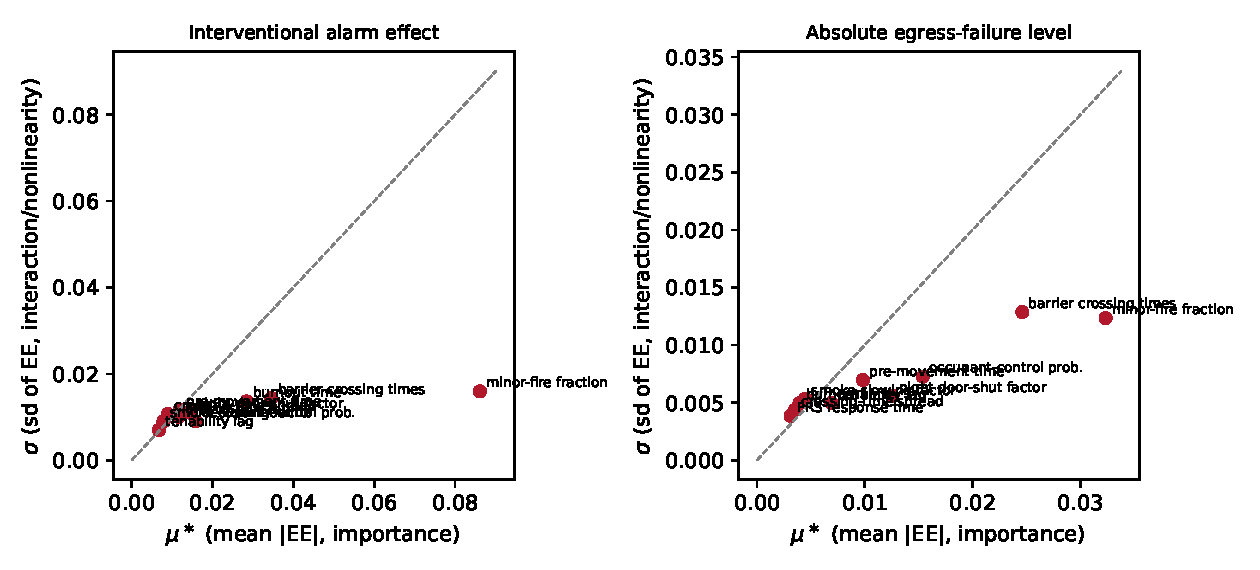
\includegraphics[width=0.92\linewidth]{figures/morris.pdf}
  \caption{Morris elementary-effects screening of the ten \emph{eng} simulator
  assumptions, for the interventional alarm effect (left) and the absolute
  evacuation-failure level (right). Each point is one assumption; $\mu^\ast$
  (horizontal) is its importance and $\sigma$ (vertical) its
  interaction/nonlinearity. The minor-fire fraction and crossing-time scale are
  the stiff directions for both outputs; burnout time is additionally stiff for
  the alarm effect (left) but sloppy for the absolute level (right). The
  interventional alarm effect stays protective and the archetype ranking fixed
  (Kendall $\tau\ge0.90$) across all $220$ design points.}
  \label{fig:morris}
\end{figure}

\section{Results}
\label{sec:results}

We instantiate the framework of Section~\ref{sec:model} in three fitted
components --- a spatial occurrence model ($P(I)$), record-level consequence
models ($P(S\mid I)$, $P(\text{casualty}\mid I)$), and the archetype simulation
surrogate ($P(E_f\mid S,I)$) --- and then assemble them into the risk
decomposition of Equation~\eqref{eq:risk}. Every number below is a held-out or
out-of-time evaluation; in-sample fit is not reported.

\subsection{Fire occurrence}
\label{sec:results-occurrence}

We model dwelling-fire counts per LSOA-year as a hierarchical negative-binomial
(NB) regression over all 33{,}755 English LSOAs, with a household-count exposure
offset, ten standardised covariates, a linear time trend, and a random intercept
for each of the 44 FRS areas. Full No-U-Turn Sampler (NUTS) sampling on the
202{,}530-row training frame is infeasible on CPU: the step size collapses
against a stiff posterior geometry under non-centred, centred and
QR-orthogonalised parameterisations alike (to $5\times10^{-7}$ in the best
case). The exact full-data posterior is nevertheless recovered without
sampling, by Pareto-smoothed importance sampling over a Laplace proposal
(Section~\ref{sec:model}): the smoothing diagnostic $\hat{k}=0.33$ certifies
the correction, with an importance-sampling effective sample size of
$\sim$16{,}900 from 50{,}000 draws, and the result agrees with an exact NUTS
fit on a stratified subsample of $\sim$10{,}000 LSOAs, full-data ADVI and
full-data MLE. Calibration is evaluated on the full held-out
population (all 33{,}755 LSOAs). Training uses FY 2017/18--2022/23; FY 2023/24
and 2024/25 are held out.

That the Laplace-plus-PSIS construction recovers the \emph{posterior}, and not
merely a well-behaved proposal, rests on the posterior being close to the Gaussian
the Laplace step assumes --- which we verify directly rather than take on faith from
$\hat{k}$ alone. Across all 58 unconstrained coordinates the importance-weighted
posterior is empirically near-Gaussian: the maximum absolute skewness is 0.13
(median 0.04) and the maximum excess kurtosis 0.33 (median 0.07), the mild
departures Bernstein--von Mises predicts at roughly 3{,}500 observations per
parameter (202{,}530 rows over 58 coordinates). A multimodality probe finds no
competing mode --- six L-BFGS optimisations from widely dispersed starts
(perturbation SD 2 in the unconstrained space) all converge to a single optimum,
agreeing to $3\times10^{-5}$ in objective value and $8\times10^{-4}$ in location.
The honest caveat sits at the tail of the hierarchy: rows per fire-and-rescue
service range from 6 (Isles of Scilly) to a median of 3{,}444, so the smallest
service effects remain partially prior-informed --- yet their marginals still fall
inside the skewness bound above, and this partial pooling is the intended shrinkage
of the hierarchical model, not a failure of the asymptotics. Finally, $\hat{k}$ is
itself a sensitive detector of proposal--posterior mismatch --- heavy tails or a
missed mode inflate it --- so $\hat{k}=0.33$ corroborates the near-Gaussian geometry
established above rather than serving as its sole warrant.

Because dwelling-fire counts per LSOA-year are small (mean $\approx0.8$, mostly
0--2), raw central-interval coverage structurally over-covers; the correct
discrete-count calibration notion is the randomised probability integral
transform (PIT), which is Uniform$(0,1)$ under calibration. On that metric the
negative-binomial model is well calibrated and beats an equal-mean Poisson on both
held-out years: from the exact full-data posterior, randomised coverage of
0.504 / 0.901 against nominal 0.50 / 0.90 in
2023/24 (and 0.495 / 0.899 in 2024/25), with a PIT Kolmogorov--Smirnov (PIT--KS)
distance of 0.0045 versus the Poisson's 0.0145 (subsample track). It also improves markedly on an
intercept-only null in held-out
log predictive density ($-1.101$ vs $-1.173$ per LSOA-year in 2023/24), confirming
that the covariate and service structure carry genuine predictive signal and that
overdispersion beyond Poisson is real, if moderate at this aggregation.
Figure~\ref{fig:occ-cal} shows the reliability curve and PIT histogram.

Covariate effects (Table~\ref{tab:occ-forest}, exact full-data posterior) are
reported as rate ratios per one-standard-deviation (SD) increase. Overall
deprivation dominates: a one-SD rise in the IMD score raises the dwelling-fire
rate by 32\% (rate ratio 1.322, 95\% credible interval (CrI) [1.310, 1.334]).
Building form (\% flats, 1.117) and
the health-deprivation domain (1.086) are the next strongest signals; \% privately
rented carries the weakest signal of any covariate (1.014 --- its interval now
excludes 1 at full-data precision, but the effect is negligible against
deprivation's 32\%) once deprivation and form are controlled. The domain coefficients are \emph{conditional} on overall IMD
(with which they are collinear, e.g.\ $r\approx0.81$ for the health domain) and
should not be read as marginal effects. This spatial gradient reproduces the
established relationship between deprivation and fire incidence
(Figure~\ref{fig:occ-decile}): predicted and observed dwelling-fire rates fall
monotonically from roughly 2.1 to 0.6 fires per 1{,}000 households across
deprivation deciles. Calibration is slightly worse in 2024/25 (PIT--KS 0.029):
the linear trend estimated through 2022/23 does not fully capture that year's
steeper decline, so the model marginally over-predicts it --- an honest
forward-forecast limitation, with coverage still on target.

\begin{table}[htbp]
  \centering
  \caption{Occurrence-model covariate effects: rate ratio per $+1$\,SD, with
  95\% credible interval; exact full-data posterior (Laplace + PSIS, all
  202{,}530 training rows). Deprivation is the dominant driver.}
  \label{tab:occ-forest}
  \small
  \begin{tabular}{@{}lcc@{}}
    \toprule
    Covariate & Rate ratio & 95\% CrI \\
    \midrule
    IMD score (overall deprivation) & 1.322 & [1.310, 1.334] \\
    \% flats (Census)               & 1.117 & [1.109, 1.126] \\
    Health-deprivation domain       & 1.086 & [1.075, 1.097] \\
    \% overcrowded                  & 1.047 & [1.039, 1.055] \\
    Living-environment domain       & 1.044 & [1.034, 1.054] \\
    \% lone-person aged 66+         & 1.043 & [1.037, 1.050] \\
    \% dwellings pre-1919 (EPC)     & 1.027 & [1.017, 1.037] \\
    \% converted flats              & 1.025 & [1.019, 1.031] \\
    \% electric main heat           & 1.017 & [1.009, 1.024] \\
    \% privately rented             & 1.014 & [1.005, 1.022] \\
    \bottomrule
  \end{tabular}
\end{table}

\begin{figure}[htbp]
  \centering
  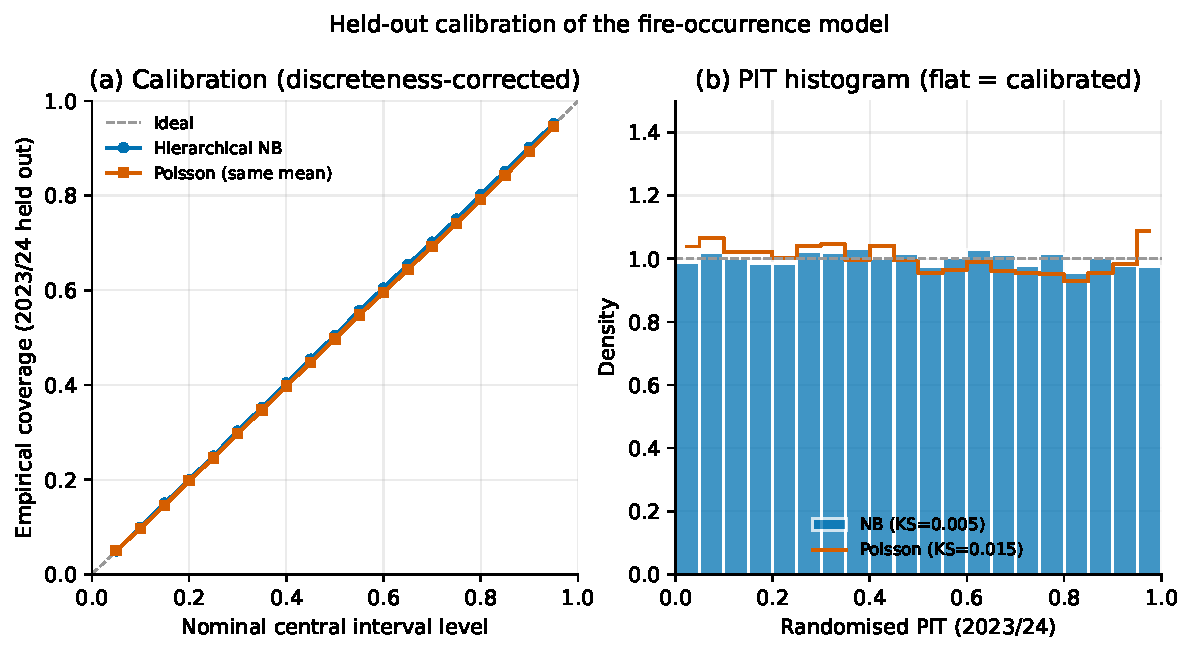
\includegraphics[width=0.8\linewidth]{figures/occ_calibration.pdf}
  \caption{Held-out calibration of the occurrence model (FY 2023/24): coverage
  of central posterior-predictive intervals (left) and randomised-PIT histogram
  (right). The PIT is close to Uniform, indicating good discrete-count
  calibration.}
  \label{fig:occ-cal}
\end{figure}

\begin{figure}[htbp]
  \centering
  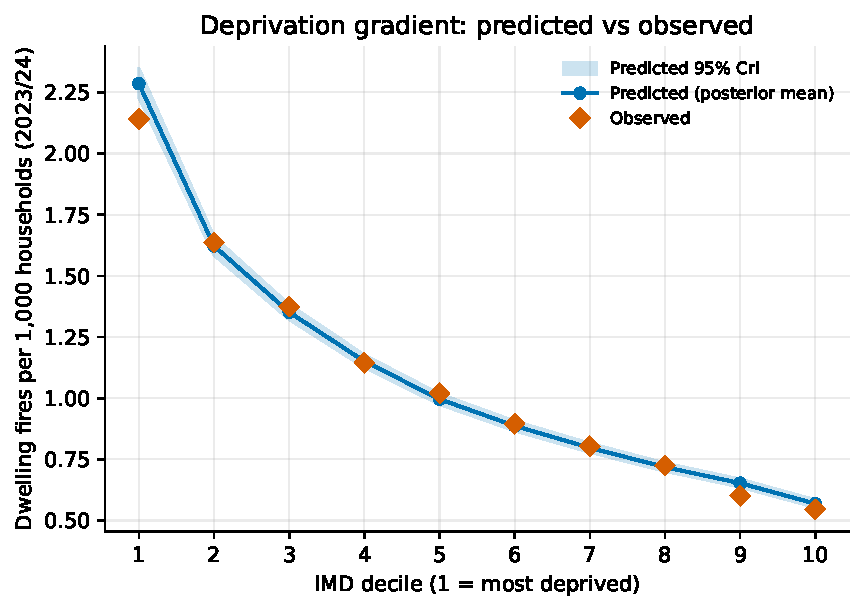
\includegraphics[width=0.55\linewidth]{figures/occ_decile_gradient.pdf}
  \caption{Dwelling-fire rate per 1{,}000 households by IMD decile, predicted
  vs observed. The monotone deprivation gradient is reproduced. Covariate rate
  ratios are in Table~\ref{tab:occ-forest}.}
  \label{fig:occ-decile}
\end{figure}

\paragraph{Robustness (full-data, ablation, spatial, subgroups).}
Three checks confirm the model. The exact full-data posterior above is
corroborated by an independent full-data ADVI refit, which
reproduces every rate ratio to within 0.022 and \emph{strengthens} the
overdispersion result --- the equal-mean Poisson undercovers badly (50\% interval
covers 0.401) while the negative binomial stays on target (0.503 / 0.901). An
ablation ladder (Table~\ref{tab:ablation}) shows deprivation is by far the largest
single gain, the EPC covariate adds essentially nothing at LSOA level, and a
Besag--York--Molli\'e (BYM2) spatial random effect removes the residual spatial
autocorrelation the service intercepts leave (Moran's $I$ falls $0.059\to-0.086$) for
only a small held-out gain --- real but modest, and this M5 specification is preferred
over the rejected quadratic-year M6. And calibration holds \emph{within} subgroups:
held-out PIT--KS stays near 0.01 across IMD quintiles, urban/rural strata and
\%-flats tertiles, with median 0.039 across the 43 service areas.

\begin{table}[htbp]
  \centering
  \caption{Occurrence ablation ladder (full-data variational fits, so M5 point
  estimates differ slightly from the exact posterior of
  Table~\ref{tab:occ-forest}), held-out
  2023/24. Deprivation dominates; the EPC covariate adds nothing at LSOA level; the
  intrinsic-conditional-autoregressive (ICAR)-based BYM2 spatial effect is real but
  modest; the preferred model is M5. Log-score is NB held-out log predictive density
  (higher is better).}
  \label{tab:ablation}
  \small
  \begin{tabular}{@{}lcccc@{}}
    \toprule
    Rung & Log-score & PIT--KS & cov50 & cov90 \\
    \midrule
    M0 intercept + trend        & $-1.1725$ & 0.0056 & 0.506 & 0.902 \\
    M1 + deprivation            & $-1.1155$ & 0.0047 & 0.504 & 0.900 \\
    M2 + building form (Census) & $-1.1024$ & 0.0044 & 0.504 & 0.902 \\
    M3 + EPC covariate          & $-1.1024$ & 0.0045 & 0.503 & 0.902 \\
    M4 + service random effect  & $-1.1000$ & 0.0039 & 0.502 & 0.901 \\
    \textbf{M5 + BYM2 spatial (preferred)} & $-1.0976$ & 0.0053 & 0.495 & 0.898 \\
    M6 + quadratic year (rejected) & $-1.0963$ & 0.0146 & 0.505 & 0.904 \\
    \bottomrule
  \end{tabular}
\end{table}

\subsection{Consequence severity}
\label{sec:results-casualty}

Two record-level outcomes are modelled from the 451{,}172 dwelling-fire records by
hierarchical Bayesian logistic regression, each with an FRS-level random intercept.
\emph{Serious spread} is fire leaving the room of origin (a direct proxy for
compartmentation failure); \emph{any-casualty} is the data-protected binary
casualty indicator (fatalities cannot be separated from non-fatal casualties at
record level). The models are fit by \emph{exact} NUTS on all 451{,}172 records
--- no subsampling --- trained on FY 2010/11--2022/23 ($n=400{,}250$) and
evaluated out-of-time on 2023/24--2024/25 ($n=50{,}922$), with every reported
fixed effect converged cleanly ($\hat{R} \le 1.02$, zero divergences). A
fiscal-year-stratified subsample fit ($n=29{,}999$) and an independent
maximum-likelihood (MLE) fit on the full records serve as cross-checks under the
two-track protocol of Section~\ref{sec:model}, reproducing the same effect signs
and comparable magnitudes. The current specification adds an
FRS-year \emph{response-time context} covariate --- the mean total call-to-arrival
delay per FRS and fiscal year from FIRE1001, joined exactly to every incident (0\% unmatched) and
standardised (1\,SD $\approx 1.23$ minutes about a 7.71-minute mean). Both models
are well calibrated out-of-time: expected calibration error (ECE) is 0.0096 for
spread and 0.0108 for casualty, and held-out area under the
receiver-operating-characteristic curve (AUC) is 0.752 and 0.685 respectively
(Figure~\ref{fig:cons-cal}); per-service interval coverage is discussed under
robustness below.

Response time itself carries only a weak, non-robust signal and must be read as an
\emph{ecological} exposure, not an incident-level measurement: it varies only at
FRS$\times$year resolution, so with the FRS random intercept absorbing between-area
differences it is identified largely from within-FRS year-to-year variation and is
partly entangled with the secular fiscal-year trend. On the subsample the casualty
odds ratio (OR) per $+1$\,SD is 0.851 (95\% CrI [0.777, 0.931]) and the spread OR
0.922 ([0.851, 0.993]); but on the full 451{,}172 records the spread effect
\emph{flips sign} (OR 1.052, [1.018, 1.084]) while casualty stays below one
(0.944, [0.915, 0.973]). We therefore report no directional response-time effect on spread, and read
the (still ecological, non-causal) casualty association only weakly; the covariate is
retained as a control, not a finding.

The headline effect is the alarm ladder (Table~\ref{tab:alarm}). For serious
spread the signal is clean and mechanistically sensible: relative to a working
alarm, a fire with \emph{no} alarm has 1.65 times the odds of spreading beyond the
room of origin (OR 1.653, 95\% CrI [1.610, 1.693]), and an alarm present that did
not raise the alarm carries the highest odds of all (OR 2.401). Detection cuts
spread. The casualty model, however, shows the no-alarm odds ratio falling
\emph{below} one (OR 0.786, [0.766, 0.804]). This sign flip is not an alarm being
harmful; it is the expected observational confound. A dwelling fire only produces a
casualty when someone is present and the fire is serious, and those same conditions
are what make an installed alarm sound --- so alarm operation is correlated with
exactly the occupancy and severity that raise casualty risk. Figure~\ref{fig:dag}
draws this backdoor path explicitly. The record-level data
cannot by itself identify the causal casualty-prevention effect; it identifies
adjusted associations. We report both outcomes precisely because the contrast ---
a clean detection$\to$spread signal alongside a confounded casualty association ---
is the motivating case for the latent-state layer of Section~\ref{sec:model},
whose job is to de-confound occupancy from detection. Reassuringly, the alarm
ladder is essentially unchanged by adding the response-time covariate (assessed on
the subsample track: the no-alarm spread OR moves 1.699$\to$1.701 and the no-alarm
casualty OR is unchanged) while calibration slightly improves, so the alarm
signal is robust to the new covariate. Other effects are large and interpretable:
chip/fat-pan fires multiply casualty odds by 3.25, lone pensioners by 2.21, and
night ignition by 1.83; purpose-built high-rise flats have the lowest spread odds
of any dwelling type (OR 0.378 vs houses), consistent with their compartmentation.

\begin{figure}[htbp]
  \centering
  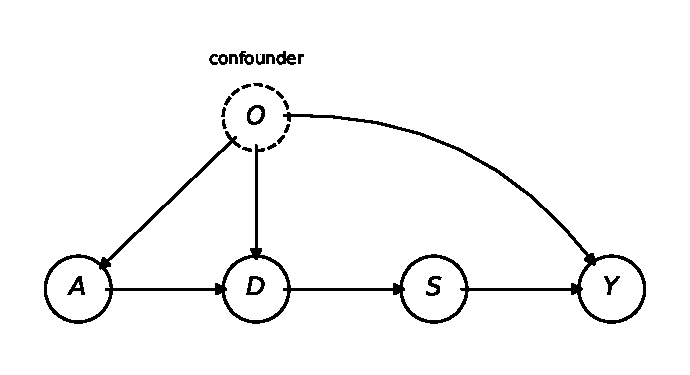
\includegraphics[width=0.55\linewidth]{figures/dag.pdf}
  \caption{Causal structure behind the alarm--casualty association. Occupancy $O$
  (dashed, the confounder) opens the backdoor path $A \leftarrow O \rightarrow Y$:
  occupied, well-maintained dwellings both carry a working alarm ($O\rightarrow A$)
  and contain someone who can be harmed ($O\rightarrow Y$), and present occupants
  themselves aid detection ($O\rightarrow D$), while the alarm reaches casualties
  only along the causal chain $A\rightarrow D\rightarrow S\rightarrow Y$ (alarm $A$,
  detection $D$, severity/spread $S$, casualty $Y$). An adjusted no-alarm casualty
  odds ratio below one is the expected signature of this structure --- alarm
  operation tracks the very occupancy that raises casualty risk --- rather than a
  protective effect of \emph{removing} alarms. The record-level data identify
  adjusted associations along this graph, whereas the intervention effect requires
  the do-operator treatment referenced in Section~\ref{sec:model}.}
  \label{fig:dag}
\end{figure}

\begin{table}[htbp]
  \centering
  \caption{Alarm ladder: odds ratios (95\% CrI) for each alarm state versus a
  working alarm (present and raised), adjusted for dwelling type, cause, ignition,
  occupancy, time, year, response time and FRS; exact NUTS posterior on all
  451{,}172 records. Detection lowers spread; the
  casualty column is confounded by occupancy (see text).}
  \label{tab:alarm}
  \small
  \begin{tabular}{@{}lcccc@{}}
    \toprule
    & \multicolumn{2}{c}{Serious spread} & \multicolumn{2}{c}{Any casualty} \\
    \cmidrule(lr){2-3}\cmidrule(lr){4-5}
    Alarm state vs.\ working & OR & 95\% CrI & OR & 95\% CrI \\
    \midrule
    Absent                       & 1.653 & [1.610, 1.693] & 0.786 & [0.766, 0.804] \\
    Present, did not operate      & 1.116 & [1.083, 1.148] & 0.789 & [0.769, 0.810] \\
    Present, did not raise alarm  & 2.401 & [2.329, 2.474] & 1.196 & [1.162, 1.230] \\
    \bottomrule
  \end{tabular}
\end{table}

\begin{figure}[htbp]
  \centering
  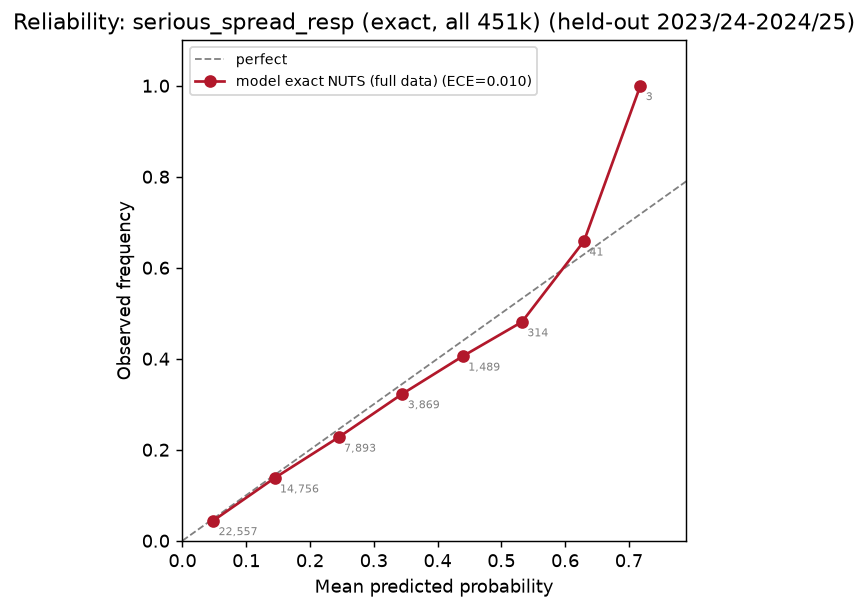
\includegraphics[width=0.7\linewidth]{figures/cons_reliability_spread.png}
  \caption{Out-of-time reliability curve for the serious-spread model
  (exact full-data NUTS, response-time specification, FY 2023/24--2024/25),
  ECE 0.0096. Predicted probabilities track observed frequencies across bins.}
  \label{fig:cons-cal}
\end{figure}

\paragraph{Robustness (proper scores, full data, subgroups).}
Because the area under the ROC curve alone is a weak test for rare outcomes, we also
report strictly proper scores (Table~\ref{tab:proper}): the hierarchical model beats an
intercept-only baseline decisively on the Brier score, mean log score and
precision--recall AUC (PR-AUC), matches a plain logistic while adding calibrated
uncertainty, and sits well above the PR-AUC base-rate floors ($\approx0.15$ / $0.13$).
The exact full-data posterior agrees with the subsample track, full-data ADVI and
full-data MLE on every headline effect (no-alarm casualty OR $0.758\to0.786$,
spread $1.70\to1.65$), and its $\sim$4$\times$ tighter intervals resolve two
subsample artefacts: the deliberate-cause casualty OR collapses from a wide,
nominally significant 3.04 [1.05, 10.6] to a clean null (1.12, [0.92, 1.38]), and
the response-time spread coefficient settles at the sign discussed above. One
honest caveat surfaces at scale: the full-data fits undercover per-FRS held-out
counts (0.81 for spread and 0.65 for casualty under exact NUTS, versus 1.00/0.93
on the subsample), and since the \emph{exact} sampler undercovers too this is a
real FRS-overdispersion gap (out-of-time drift and within-service heterogeneity a
single intercept misses), not a variational artefact --- fixed effects are best
estimated from the full data, while per-service predictive intervals from the
tighter full-data posterior should be read as anti-conservative and a
random-slope extension is future work. Calibration broadly holds \emph{within} alarm,
dwelling-type and time-of-day subgroups (most subgroup expected calibration errors of
the same $0.01$--$0.02$ order as the marginal figure, with larger wobbles at
small-$n$ cells such as bungalows, ECE $0.09$ at $n{=}189$).

\begin{table}[htbp]
  \centering
  \caption{Held-out proper scores for the consequence models versus an intercept-only
  baseline (subsample held-out, $n=3{,}386$). Lower Brier and log score are better;
  higher PR-AUC and ROC-AUC are better. The hierarchical model ranks rare events well
  above the base-rate floor.}
  \label{tab:proper}
  \small
  \begin{tabular}{@{}llcccc@{}}
    \toprule
    Outcome & Model & Brier & Log score & PR-AUC & ROC-AUC \\
    \midrule
    Casualty       & Hierarchical    & 0.1205 & 0.3984 & 0.245 & 0.659 \\
    Casualty       & Intercept-only  & 0.1250 & 0.4166 & 0.146 & 0.500 \\
    Serious spread & Hierarchical    & 0.1041 & 0.3446 & 0.318 & 0.757 \\
    Serious spread & Intercept-only  & 0.1160 & 0.3939 & 0.134 & 0.500 \\
    \bottomrule
  \end{tabular}
\end{table}

\subsection{Interaction structure: who gains most from an alarm}
\label{sec:results-interactions}

Does the alarm benefit differ by occupancy, and the night penalty by dwelling type?
We add two interactions to the consequence model --- alarm$\times$occupancy and
night$\times$dwelling-type --- and, because interaction cells are noisy, hold them to
a strict discipline: a joint likelihood-ratio (LR) test of each interaction block on
the full data, Benjamini--Hochberg false-discovery-rate (BH-FDR) control across cells,
and a dual gate that calls a cell robust only if it clears \emph{both} the Bayesian
95\% credible interval and the full-data maximum-likelihood interval with the same
sign. Of 68 tested cells, the robust ones are 8 (spread) and 5 (casualty) in
alarm$\times$occupancy and 2 (casualty) in night$\times$dwelling.

The spread channel --- the cleaner, less-confounded detection signal --- shows a
genuine \emph{occupancy gradient} in the value of a working alarm
(Figure~\ref{fig:int-ame}). The no-alarm-versus-working spread odds ratio runs from
about 3.30 [3.04, 3.57] for a lone person over pensionable age --- roughly double the
pooled 1.65 --- down to indistinguishable-from-none for families with children (who
have waking occupants to detect a fire). Lone pensioners, lone under-pensioners and
older couples all sit robustly above the pooled penalty (the cell probabilities are
reported as adjusted average marginal effects, AME). By contrast the night effect on
spread is a \emph{whole-stock} phenomenon: none of the seven dwelling deviations from
the house reference clears both gates, so no building form --- HMOs and converted
flats included --- is disproportionately worse at night once the shared night penalty
is removed. The interaction terms do not degrade calibration (held-out ECE
0.012--0.014). The targeting consequence is drawn out in
Section~\ref{sec:discussion}: the alarm benefit should be occupancy-modulated toward
lone pensioners, while night warrants no dwelling-specific multiplier.

\begin{figure}[htbp]
  \centering
  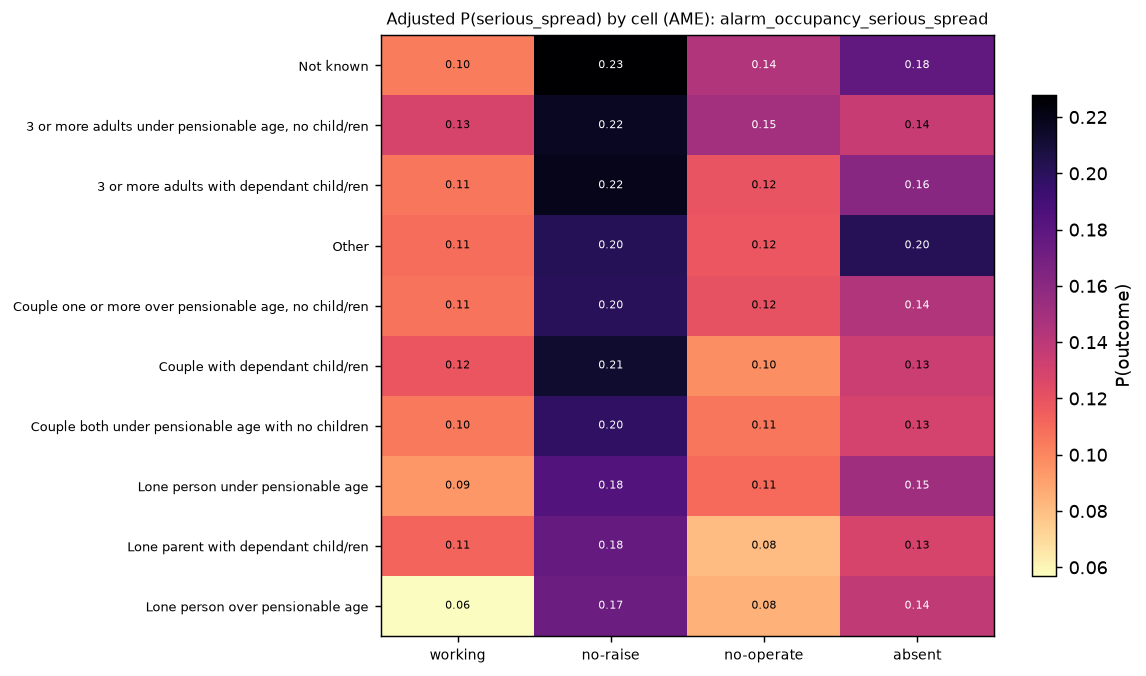
\includegraphics[width=0.82\linewidth]{figures/int_ame_alarm_occupancy.png}
  \caption{Adjusted probability of serious spread by occupancy type (rows) and alarm
  state (columns), from the alarm$\times$occupancy interaction. The no-alarm spread
  penalty is largest for lone pensioners, who gain the most containment from a working
  alarm.}
  \label{fig:int-ame}
\end{figure}

\subsection{Simulation and surrogate}
\label{sec:results-sim}

The evacuation-failure factor $P(E_f\mid S,I)$ comes from the archetype simulator
of Section~\ref{sec:surrogate}, run for 420{,}000 Monte Carlo ignitions (10{,}000
per archetype~$\times$~alarm~$\times$~time-of-day cell, fixed seed). Every parameter
is declared in a single assumptions registry with a provenance tag (calibrated to
data, consistent with PD~7974 and Society of Fire Protection Engineers (SFPE)
practice, grounded in the literature, or a transparent engineering estimate), so
the model is auditable rather than a black box. Table~\ref{tab:sim} gives the
headline night-time per-occupant evacuation-failure probabilities.

\begin{table}[htbp]
  \centering
  \caption{Per-occupant $P(\text{evacuation failure}\mid\text{ignition})$ at
  night, by archetype and alarm state (Monte Carlo, 95\% confidence intervals (CIs)
  in the full results).
  A working alarm roughly halves failure in most archetypes; the care home is the
  exception (see text).}
  \label{tab:sim}
  \small
  \begin{tabular}{@{}lccc@{}}
    \toprule
    Archetype & no alarm & alarm not working & working alarm \\
    \midrule
    detached house & 0.385 & 0.370 & 0.249 \\
    terraced house & 0.404 & 0.396 & 0.242 \\
    low-rise flat  & 0.141 & 0.132 & 0.049 \\
    high-rise flat & 0.071 & 0.068 & 0.012 \\
    HMO            & 0.364 & 0.355 & 0.262 \\
    care home      & 0.163 & 0.165 & 0.168 \\
    mixed use      & 0.181 & 0.176 & 0.070 \\
    \bottomrule
  \end{tabular}
\end{table}

The care home is the informative exception: its evacuation-failure rate barely
moves with alarm state (0.163 / 0.165 / 0.168 at night), because its bottleneck is
occupant \emph{mobility}, not \emph{detection} --- a 75\% mobility-impaired
population with long pre-movement times cannot exploit earlier warning under a
full-evacuation assumption. Detection helps where egress is fast (flats, houses);
it does not where egress is slow. This is exactly the kind of archetype-specific
mechanism the surrogate is meant to expose.

Against the observed dwelling-fire statistics the simulator is \emph{loosely}
calibrated --- we target orderings and magnitudes, not exact matches --- and the
orderings hold. Spread beyond the room of origin ranks working alarm $<$ not
working $<$ none (simulation 0.100 / 0.185 / 0.184 vs data 0.079 / 0.146 / 0.185)
and night $>$ day (0.176 vs 0.137, data 0.207 vs 0.117); the compartmentation
ordering is strong, with purpose-built flats almost never spreading beyond the
floor of origin. The one acknowledged discrepancy is that multi-storey
\emph{houses} over-predict spread beyond the floor (simulation $\approx$0.13 vs
data 0.05), because an open internal stair lets fire climb too readily; flats match
closely. The simulator also independently reproduces the same casualty confound
seen in the record data --- observed casualty rate is \emph{highest} with a working
alarm --- while its causal $P(E_f)$ correctly \emph{decreases} with a working
alarm, which is the interventional quantity the risk model needs.

The new building-type benchmarks (FIRE0301/0304) give the care-home and mixed-use
archetypes their first real calibration targets, and they validate the
institutional archetypes with no change to the simulator's parameters. The
care-home archetype's spread-beyond-room rate (0.079) matches the observed
`communal living' class almost exactly (0.082) and sits far below the commercial
classes (retail 0.203, food-and-drink 0.225), confirming its institutional
compartmentation is at the right level. On consequence, communal-living buildings
have the highest casualty-per-fire of the residential-type classes (0.110), and the
care-home archetype's per-occupant evacuation-failure rate (0.156) is the right
order of magnitude, overstating the observed per-occupant casualty rate by roughly
$1.4\times$; the building-level $P(\geq 1\ \text{occupant fails})$ of 0.528
overstates by construction far more ($\sim$$4.8\times$) --- both are the
no-staff-assist, stay-put- and sprinkler-free full-evacuation upper bound flagged
as a limitation, now quantified against data. Separately, the smoke-alarm operation rate
$P(\text{operated}\mid\text{present}) = 0.743$ (FIRE0703) and working-alarm
ownership 0.924 (FIRE0701) confirm the \emph{structure} of the three-way alarm
split --- both a large ``working'' and a large ``present-but-failed'' population ---
but they are timing-free aggregate counts, so no detection parameter was changed.

Finally, three logistic-regression surrogates map archetype features (storeys,
occupants, compartmentation, impaired fraction, alarm state, night) to the three
consequence probabilities, recovering the Monte Carlo cell probabilities with
$R^2 = 0.861$ (spread beyond room), $0.969$ (spread beyond floor) and $0.936$
(evacuation failure), all with interpretable coefficient signs and bootstrap
prediction intervals. This surrogate is the closed-form $\mathbb{E}[C\mid I]$
engine that plugs into Equation~\eqref{eq:consequence}
(Figure~\ref{fig:sim-fail}).

\begin{figure}[htbp]
  \centering
  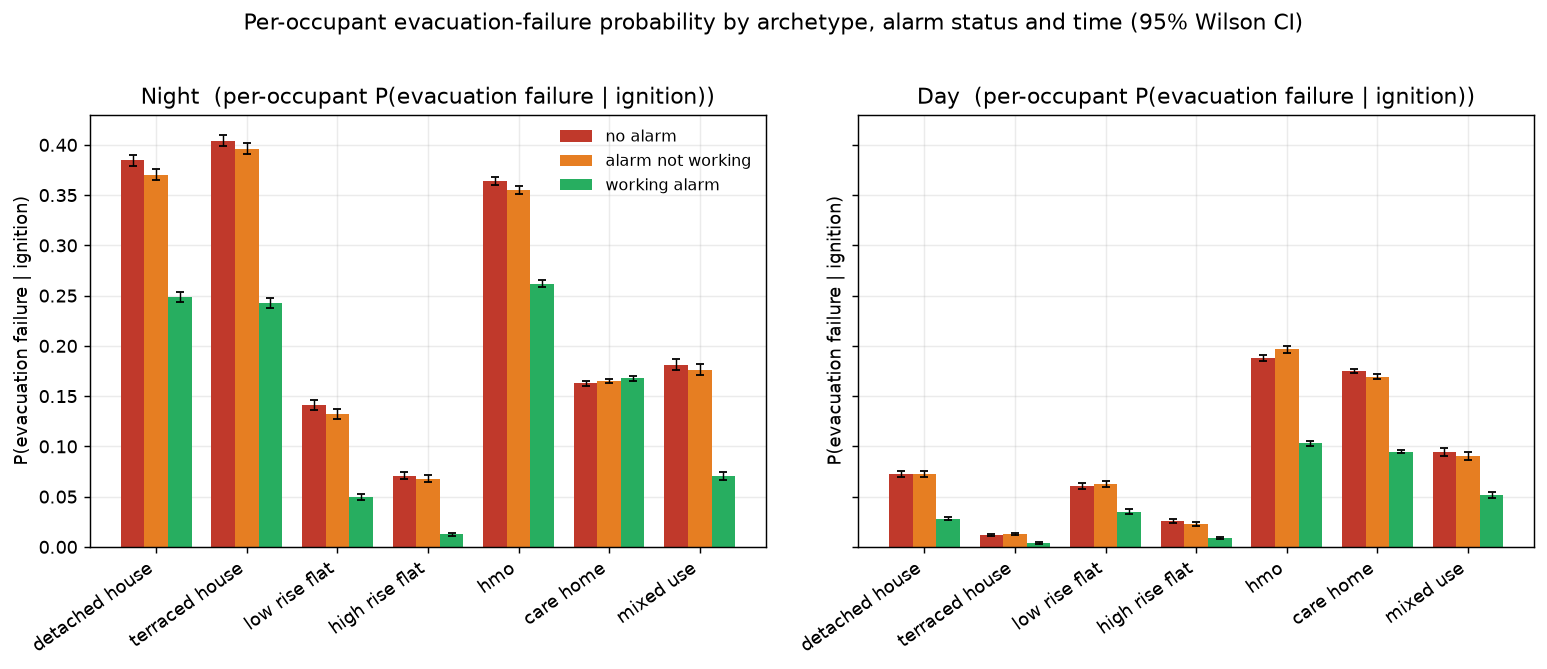
\includegraphics[width=0.82\linewidth]{figures/sim_failure_by_archetype.png}
  \caption{Per-occupant probability of evacuation failure by archetype, alarm
  state and time of day, with 95\% Monte Carlo error bars. A working alarm lowers
  failure in every archetype except the care home, whose bottleneck is mobility,
  not detection.}
  \label{fig:sim-fail}
\end{figure}

\subsection{Synthesis: a worked risk decomposition}
\label{sec:results-synthesis}

The three components combine into the posterior risk of
Equation~\eqref{eq:risk}, carrying uncertainty through each factor. Consider an
illustrative high-rise flat in a most-deprived-decile LSOA at night with no
working alarm. The occurrence model places the annual ignition probability near
the top of the deprivation gradient, $P(I)\approx 2.1\times10^{-3}$ per
household-year (Figure~\ref{fig:occ-decile}); the surrogate gives, for the
high-rise-flat archetype with no alarm at night, $P(S\mid I)\approx0.24$ and
$P(E_f\mid S,I)\approx0.071$. Composing these,
\begin{equation}
  R_b \;=\; \underbrace{P(I)}_{\approx 2.1\times10^{-3}}\;\cdot\;
  \underbrace{P(S\mid I)}_{\approx 0.24}\;\cdot\;
  \underbrace{P(E_f\mid S,I)}_{\approx 0.071}\;\cdot\;
  \mathbb{E}[L\mid\cdot]
  \;\approx\; 3.6\times10^{-5}\cdot\mathbb{E}[L\mid\cdot]\ \text{per hh-year},
  \label{eq:worked}
\end{equation}
before the loss term. Fitting a working alarm collapses the middle factor toward
$P(S\mid I)\approx0.09$ and the egress factor to $P(E_f\mid S,I)\approx0.012$, an
order-of-magnitude reduction in the evacuation-failure contribution --- the
quantitative expression of the intervention. To collapse these alarm-conditional
outputs into a single population-average consequence for a stock of mixed alarm
reliability, the surrogate's working and not-working predictions are combined using
the empirical smoke-alarm operation rate $P(\text{operated}\mid\text{present})=0.743$
(FIRE0703; Section~\ref{sec:results-sim}) as the population weight --- supplied to
the risk model rather than baked into the simulator. Crucially each factor carries a
credible interval (the occurrence posterior, the consequence-model CrIs of
Table~\ref{tab:alarm}, and the surrogate's bootstrap prediction intervals), so the
product in Equation~\eqref{eq:worked} is a \emph{distribution} over $R_b$, not a
point score, and the width of that distribution is itself the missing-evidence
signal that drives inspection prioritisation (Section~\ref{sec:model-inspection}).
These figures are illustrative of the composition rather than a calibrated
building-level prediction; building-level validation remains at the aggregate level
(Section~\ref{sec:discussion}).

\subsection{Decision layer: value of targeted prevention}
\label{sec:results-decision}

The framework exists to support decisions, so we close the analysis with a worked
value-of-inspection demonstration (contribution~4): given a \emph{fixed} prevention
budget, how much better can a fire and rescue service target it using the calibrated
posteriors than with untargeted or deprivation-only rules? This is emphatically
\emph{not} an argument against statutory fire risk assessment --- PAS~79
\citep{pas79_1_2020}, the Building Safety Act and the post-Grenfell regime are valued
safety improvements. The decision layer is a quantitative prioritisation layer that
\emph{backs} that regime with data: which homes, in which order, for a limited
budget. The policy evaluated is a real intervention --- FRS home fire-safety
(``Safe and Well'') visits that install or check a working smoke alarm --- at a fixed
budget of 100{,}000 visits across England. Four ranking rules are evaluated against
the same world (Table~\ref{tab:decision}): random, IMD-decile (current common
practice), posterior fire rate, and a full expected-benefit rule that is
uncertainty-aware and consequence-valued (rate~$\times$~$P(\text{no working
alarm})$~$\times$~$P(\text{casualty}\mid\text{fire})$~$\times$~relative risk
reduction (RRR)).

Economic values are the Home Office \emph{Economic and Social Cost of Fire}
\citep{homeoffice2023costfire}: averting one casualty-fire is worth \pounds66{,}113
(national-average severity, dominated by the rare fatality) and a working alarm
averts an assumed 20\% of a fire's \pounds14{,}009 property damage; benefits accrue
over a 10-year alarm life discounted at 3.5\% (present value (PV) multiplier 8.61)
against a \pounds55 visit cost. The alarm's causal effect is taken from the
\emph{interventional} surrogate rather than the confounded observational casualty
odds ratio (which is below one), and is cross-checked against the observational
spread signal; every causal assumption is tabled with a sensitivity sweep.

Targeting multiplies the return roughly ninefold: expected-benefit targeting returns
\pounds0.71 per \pounds1 spent versus \pounds0.078 for random allocation, and averts
3.1 casualty-fires per year against 0.34 (Table~\ref{tab:decision}). The calibrated
occurrence model also beats the
deprivation proxy by about $2.5\times$ (3.0 vs 1.2 casualty-fires averted for
posterior-risk vs IMD-decile targeting): deprivation is a genuinely strong single
proxy --- it co-varies with fire rate, the alarm gap and vulnerability at once, which
is why services use it and we treat it respectfully --- but within the deprived
deciles the calibrated model pinpoints the specific high-rate LSOAs that
random-within-decile misses. The consequence and uncertainty-aware signals add a
further modest gain (0.705 vs 0.673); they are collinear with the fire rate here, so
once the rate is modelled well they add little, and they would matter more where
consequence decouples from occurrence. The absolute return sits below
\pounds1/\pounds1 by construction: we value \emph{only} the alarm's consequence
channel and exclude the visit's fire-prevention advice and health co-benefits, so
every figure is a deliberate lower bound. The contribution is the targeting
multiplier and the uncertainty-aware decision rule, not a claim that alarm
installation pays for itself on casualties alone; a sensitivity sweep shows the break-even frontier crossing the plausible
parameter region --- reached around a \pounds30 visit cost at the base effect
size, and requiring correspondingly larger interventional effects at higher
costs (Figure~\ref{fig:decision-sens}).

\begin{table}[htbp]
  \centering
  \caption{Value of targeting a fixed 100{,}000-visit smoke-alarm budget under four
  ranking rules, evaluated against the same England-wide world. Present value over a
  10-year alarm life at 3.5\%, casualty plus property, with 90\% credible intervals
  propagated from the occurrence posterior and surrogate bootstrap.}
  \label{tab:decision}
  \small
  \begin{tabular}{@{}lrcc@{}}
    \toprule
    Policy & LSOAs & Casualty-fires averted/yr & \pounds saved per \pounds spent \\
    \midrule
    (a) Random               & 33{,}755 & 0.34 [0.33, 0.35] & 0.078 [0.076, 0.080] \\
    (b) IMD decile           & 145      & 1.19 [1.15, 1.24] & 0.274 [0.267, 0.282] \\
    (c) Posterior risk       & 127      & 3.00 [2.87, 3.14] & 0.673 [0.649, 0.697] \\
    (d) Expected benefit     & 127      & 3.13 [2.99, 3.29] & 0.705 [0.678, 0.731] \\
    \bottomrule
  \end{tabular}
\end{table}


\paragraph{Formal allocation, value of inspection, and budget size.}
The allocation is the constrained maximisation of expected averted loss of
Equation~\eqref{eq:knapsack}; because every dwelling in an LSOA shares the same
marginal value, it is a continuous knapsack whose optimum is the greedy rule (rank by
marginal value, fill from the top), and policy (d) is its Bayes action --- ranking by
posterior-mean averted loss. Reframing the visit as an inspection that resolves alarm
ownership gives the EVI of Equation~\eqref{eq:evi}, which sharpens the picture: the
prior-optimal action is to visit in only 0.04\% of dwellings (expected benefit exceeds
the \pounds55 cost almost nowhere), yet a visit \emph{would} pay in the 29.0\% of
dwellings that turn out to lack a working alarm --- so the programme's whole value lies
in \emph{finding} those homes, which is what inspection does, with total EVI over
England $\approx\pounds22.7$m. EVI is also a genuinely different ranking from expected
risk (Spearman $\rho=0.79$, versus $0.985$ for expected-benefit-versus-risk): it zeroes
out the $\sim$71\% of areas where a visit can never pay, so uncertainty-reducing
targeting is distinct from risk targeting even though the two coincide on the top LSOAs
a 100{,}000-visit budget reaches.

The headline economic result is a break-even one, and it is about concentration, not
scale. Sweeping the budget (Table~\ref{tab:budget}), a small, tightly targeted
10{,}000-visit programme clears break-even on the smoke-alarm channel alone
(\pounds1.12 per \pounds1) even on our conservative casualty-plus-property valuation;
the advantage over IMD targeting then falls from $4.4\times$ at 10{,}000 visits to
$1.4\times$ at one million as a larger programme is pushed down into lower-risk stock.
A decision-curve analysis and the visit-cost$\times$effect-size sensitivity map
(Figure~\ref{fig:decision-sens}) place the break-even frontier inside the plausible
region: cheaper visits or the upper half of the effect-size range lift the channel
above \pounds1/\pounds1.

\begin{table}[htbp]
  \centering
  \caption{Return per pound (present value, casualty plus property) by programme size
  and policy. A small, tightly targeted programme clears break-even (\pounds1.12);
  the targeting advantage over IMD decays with scale (classic diminishing returns).}
  \label{tab:budget}
  \small
  \begin{tabular}{@{}rcccc@{}}
    \toprule
    Visits & Random & IMD decile & Posterior risk & Expected benefit \\
    \midrule
    10{,}000    & 0.078 & 0.252 & 1.112 & \textbf{1.119} \\
    50{,}000    & 0.078 & 0.255 & 0.800 & 0.821 \\
    100{,}000   & 0.078 & 0.256 & 0.673 & 0.704 \\
    250{,}000   & 0.078 & 0.261 & 0.545 & 0.563 \\
    500{,}000   & 0.078 & 0.260 & 0.449 & 0.464 \\
    1{,}000{,}000 & 0.078 & 0.267 & 0.362 & 0.374 \\
    \bottomrule
  \end{tabular}
\end{table}

\begin{figure}[htbp]
  \centering
  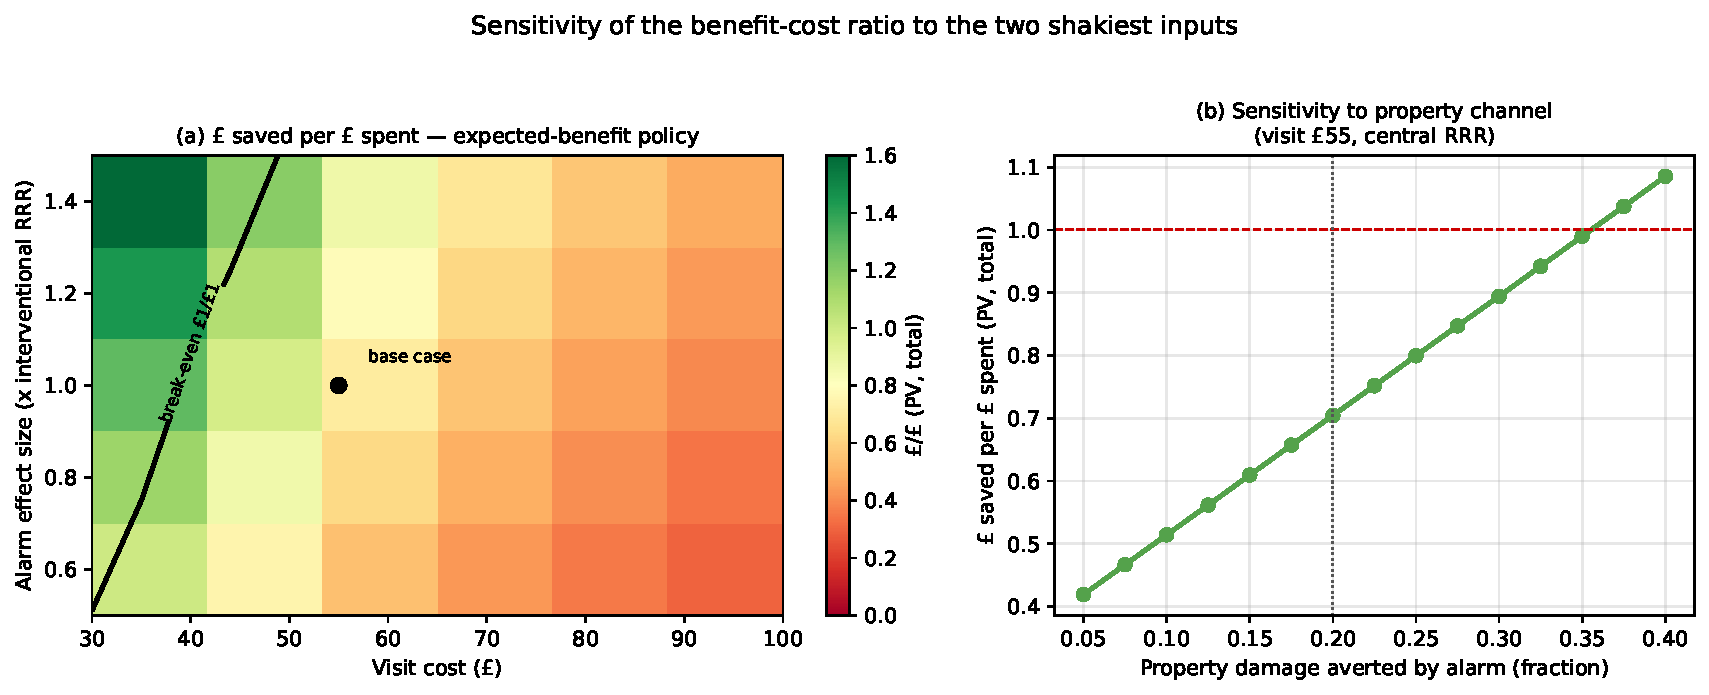
\includegraphics[width=0.78\linewidth]{figures/decision_sensitivity.pdf}
  \caption{Return per pound over visit cost (\pounds30--\pounds100) and alarm
  effect size (0.5--1.5$\times$ the interventional RRR), with the break-even contour
  and base-case marker. The frontier crosses the plausible region.}
  \label{fig:decision-sens}
\end{figure}

\paragraph{What finer geography buys: sub-LSOA concentration in London.}
The decision results above inherit the framework's granularity ceiling: the
national incident data resolve only to LSOA. London is the one fire service that
publishes incident records at finer resolution --- dwellings on a 50\,m grid ---
and a pilot on those records (90{,}318 dwelling fires, 2009--2024, with
EPC-derived dwellings per cell as exposure) shows how much that ceiling costs.
Within an average London LSOA, the top 10\% of inhabited 50\,m cells hold
\textbf{83\%} of the LSOA's dwelling fires, against 59\% expected from dwelling
density and small-count sampling noise alone (a dwelling-density multinomial
null; the honest signal is the 24-point excess). Priced with the same economics
as the policy comparison above, and evaluated \emph{out-of-sample} (cells
ranked on 2009--2020 by empirical-Bayes shrunk rates, every selected dwelling
scored at its realised 2021--2024 rate), cell-level targeting reaches dwellings
with \textbf{5.7$\times$} the fire rate of LSOA-level targeting at a
10{,}000-visit London budget --- lifting the smoke-alarm channel from
\pounds0.33 to \pounds1.88 saved per \pounds1 spent, i.e.\ above break-even
where LSOA targeting is not close (4.2--5.0$\times$ at larger budgets; a
perfect-foresight oracle reaches 11$\times$, the gap measuring how much apparent
concentration is noise). Both caveats push the estimate to be conservative: the
50\,m rounding coarsens true building-level concentration, and the $\sim$14\% of
fires falling outside EPC-covered cells are dropped from observed and null
alike (Figure~\ref{fig:london-targeting}). The implication is not that the
national model is wrong --- its calibration holds --- but that its geography
leaves roughly a sixfold value multiplier on the table, which is precisely the
case for record-level access to fine incident geography
(Section~\ref{sec:discussion}).

\begin{figure}[htbp]
  \centering
  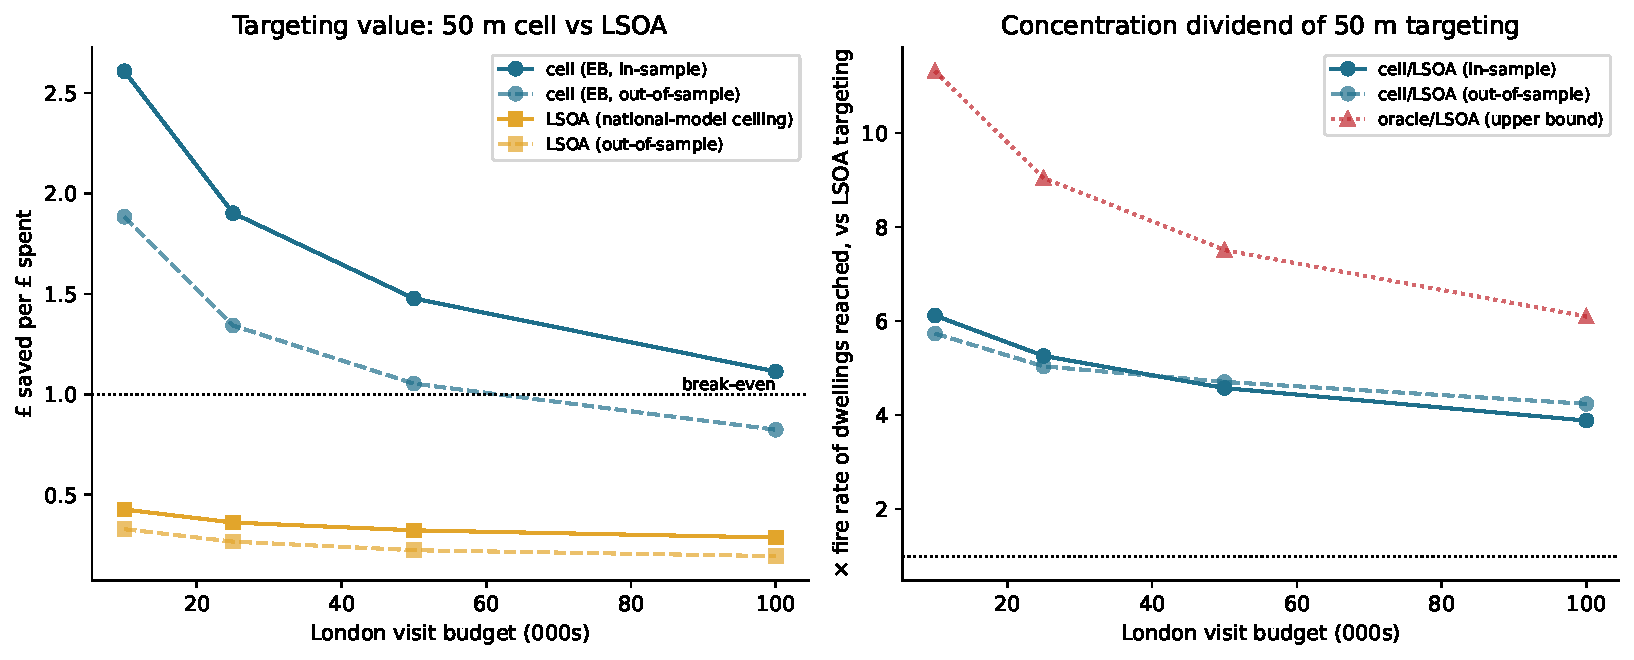
\includegraphics[width=0.85\linewidth]{figures/london_targeting.pdf}
  \caption{London pilot: out-of-sample value of sub-LSOA targeting. Cells ranked
  on 2009--2020 empirical-Bayes rates and scored on realised 2021--2024 rates;
  cell-level targeting reaches dwellings with 4.2--5.7$\times$ the fire rate of
  LSOA-level targeting across budgets, crossing break-even on the smoke-alarm
  channel alone at small budgets.}
  \label{fig:london-targeting}
\end{figure}

\subsection{Real-building stress test: Grenfell as a model-boundary case}
\label{sec:results-casestudy}

To probe how far the generic archetypes deviate from a real, exhaustively documented
building, we ground the high-rise-flat archetype against Grenfell Tower (14 June
2017), using only public evidence from the Grenfell Tower Inquiry Phase~1 report
\citep{grenfell2019phase1}. The 72 people who died are the reason this work exists;
the case study is framed in that spirit, and its purpose is to state plainly what a
population-scale interior model can and cannot represent. We rebuild the tower to its
real scale (24 storeys, six flats per floor, 120 residential flats, a single central
stair, 297 occupants present) with the same simulation engine and no change to any
parameter, and walk a one-variable-at-a-time path from the published archetype to the
real building (Table~\ref{tab:casestudy}).

The path isolates a clear finding: \emph{geometry barely matters; regime assumptions
dominate}. Placing the fire in the occupied flat --- the correct picture for the
exposed household under a stay-put design --- raises per-occupant evacuation failure
from 0.072 to 0.252 with no change in geometry. Replacing the generic 12-storey shape
with Grenfell's real 24-storey geometry then moves it only a further 2\% (0.252 to
0.258): doubling the storeys and adding flats per floor is nearly irrelevant to
whether the origin household escapes, because the single-stair topology the archetype
\emph{already} encodes is the safety-critical feature, and its compartmentation score
(1.356) essentially matches the real graph's (1.345). The catastrophe is a regime
change, not a geometry effect: losing compartmentation and forcing simultaneous full
evacuation takes per-occupant failure to 0.987 and expected fatalities from about 0.5
(one household) to about 293 (the whole building). The parameters that differ most
between archetype and reality --- the number of occupants in the evacuation problem
(2, the origin household under an intact stay-put design, vs 297, the whole building
once stay-put is revoked; per-flat occupancy is nearly identical at $\approx$2--2.5)
and storeys (12 vs 24) --- are \emph{not} the parameters that move the risk; whether compartmentation holds and
whether the building stays under stay-put are. The generic archetype is therefore a
sound geometric proxy whose one material simplification, shared by every archetype,
is that it presumes the design strategy holds.

Two honest boundaries follow. First, even in the breached case a working common alarm
with early simultaneous evacuation cuts expected fatalities from about 293 to about 4
--- the interior consequence of the post-Grenfell shift toward evacuation-alert
systems, which the model reproduces. Second, and decisively, \emph{our interior graph
has no external facade}. The mechanism that actually destroyed Grenfell --- flames
running up aluminium composite material (ACM) rainscreen cladding with polyethylene
cores and re-entering flats through failed windows on many floors at once --- lies
entirely outside a room--corridor--stair model, which is why the breached no-alarm
case predicts about 293 of 297 failing when 72 in fact died: it is a worst-case
envelope (no time-phased escape, a hard tenability cutoff), not a reconstruction. That
blind spot is not a defect to patch inside the model; it is the boundary between
population-scale interior risk ranking and the external-wall and safety-case regime
--- the combustible-cladding ban, Requirement~B4 external-fire-spread compliance
(which Grenfell failed), and the Building Safety Act's higher-risk-building regime ---
created precisely for the hazard our model cannot see. That division of labour is the
honest conclusion. Table~\ref{tab:grenfell-assumptions} makes the envelope explicit:
each simplification in the breached scenario removes a survival mechanism that
operated on the night, so every bias points the same way, and the two runs should be
read as brackets --- the event traversed from the intact regime toward the breached
one over roughly two hours, and the actual toll reflects who was still inside when
that transition completed.

Conditions (a) and (b) bracket the problem; a third condition (c) \emph{tests} it.
Feeding the model the documented Phase~1 fire timeline as an exogenous boundary
condition --- cladding involvement, an upward front of about one floor per minute,
lobby smoke-logging from $\approx$01:40, the single stair carrying significant smoke
from 02:00 --- and simulating only the egress and tenability response, with behaviour
calibrated \emph{solely} to the recorded departure anchor (``168 of 297 out by
01:50'', which the model reproduces at 176) and \emph{never} to the death toll, the
model predicts 37 expected fatalities (90\% Monte Carlo [28, 46]) against the actual
72 --- the right order of magnitude, under by about half (Table~\ref{tab:casestudy},
row (c)). This tests only the egress/tenability half of the model, since the hazard
field is imposed rather than derived. The miss is structured, not diffuse: a
five-parameter sensitivity sweep --- including the two per-floor stair-lethality
knobs that dominate the fatality count, each over its stated factor-of-two range ---
spans [12, 99] in expectation; constrained to departure curves consistent with the
observed anchor (155--185 out by 01:50), it spans [20, 73], so the true toll of 72
sits at the \emph{upper boundary} of the anchor-respecting envelope rather than
comfortably within it, and predicted fatalities rise with height as the documented
toll did. The central estimate reaches 72 only by pushing every dominant knob to its
lethal extreme; at plausible-central settings the tenability mechanics under-predict,
which localises the missing half to factors the model deliberately does not tune away:
occupant vulnerability held
at the archetype's 10\% impaired fraction (Grenfell's dead were disproportionately
disabled, elderly and children), coarse rescue and smoke modelling, and stay-put
maintained beyond survivable conditions --- the human and behavioural failures the
Inquiry identified. An honest, un-tuned under-prediction of this shape is more
informative than a fitted hit: the geometry and tenability mechanics are sound, and
the missing half lives in vulnerability and policy, not in the model's physics.

\begin{table}[htbp]
  \centering
  \caption{Breached-scenario assumptions vs the recorded event (Grenfell Tower
  Inquiry Phase 1). Every simplification removes a survival mechanism, so the
  scenario is a one-sided worst-case envelope: it predicts $\approx$293 of 297
  failing where 72 died. The intact-compartmentation run ($\approx$0.5 expected)
  is the opposite envelope, assuming the stay-put design works perfectly.}
  \label{tab:grenfell-assumptions}
  \small
  \begin{tabular}{p{0.30\linewidth}p{0.38\linewidth}p{0.22\linewidth}}
    \hline
    Model assumption (breached run) & What happened on the night & Bias on fatalities \\
    \hline
    Compartmentation lost building-wide at ignition &
    Progressive failure over $\sim$1--2\,h as the facade fire re-entered floor by
    floor & overstates \\
    Unaided self-evacuation only &
    Dozens rescued or assisted by firefighters & overstates \\
    Occupants move only when alerted, uniform compliance &
    168 of 297 had left by 01:50, many against stay-put advice, before its 02:47
    revocation; deaths concentrated among those who remained longest & overstates \\
    Stair degrades with the compartment loss &
    The single stair remained partially passable for hours despite smoke-logging &
    overstates \\
    Hard tenability cutoff, no refuge or relocation &
    Some occupants moved between flats and survived long after lobbies
    smoke-logged & overstates \\
    \hline
  \end{tabular}
\end{table}

\begin{table}[htbp]
  \centering
  \caption{Deviation path from the published archetype to real Grenfell geometry
  (rows a: night, no alarm). Per-occupant evacuation-failure probability and expected
  number of occupants failing to escape. Geometry moves the exposed-household risk by
  only 2\%; the regime change (lost compartmentation + full evacuation) moves it by
  two orders of magnitude. Row (c) is the as-unfolded hindcast under the imposed
  Phase~1 timeline (per-occupant fatality; predicted vs actual 72).}
  \label{tab:casestudy}
  \small
  \begin{tabular}{@{}lrcc@{}}
    \toprule
    Configuration & Occ. & $P(\text{fail}\mid\text{occ.})$ & $\mathbb{E}[\text{n fail}]$ \\
    \midrule
    Generic archetype (as published)          & 2   & 0.072 & 0.14 \\
    Generic geometry, fire in occupied flat    & 2   & 0.252 & 0.50 \\
    Grenfell geometry, intact (stay put)       & 2   & 0.258 & 0.52 \\
    Grenfell breached, full evacuation         & 296 & 0.987 & 292.5 \\
    \midrule
    (c) As-unfolded hindcast (imposed timeline) & $\sim$288 & 0.128 & 37 (actual 72) \\
    \bottomrule
  \end{tabular}
\end{table}

\subsection{Instantiating the inspection layer on real assessments}
\label{sec:results-latent}

The paper's proposed inspection-as-noisy-observation layer
(Section~\ref{sec:model}) is here fitted to real data for the first time: a corpus of
1{,}441 published fire risk assessments over 653 Camden council estates
\citep{camden_fra}, linked to London Fire Brigade primary-fire histories
\citep{lfb_incidents}. What is \emph{established} is the apparatus, not a positive
validity claim, and we state each part plainly.

\emph{The measurement model fits coherently.} A joint latent-factor model over the 653
estates recovers a single continuous latent deficit state $\theta$ whose measurement
model is the FRA indicators. They load coherently on it --- priority-A and priority-B
action counts, overall rating and the compartmentation, electrical and alarm flags all
move together (only the higher-risk-building-specific external-wall flag is near zero)
--- so $\theta$ is a well-defined ``assessed-deficiency'' state. Of the between-estate
log fire-rate variance attributed to $\theta$ plus the public deprivation covariate,
$\theta$ carries a median 94\%: the latent read off the inspection dominates the IMD
covariate in explaining where estate fire rates differ.

\emph{The posterior update works numerically.} For a worked single block (six flats,
most-deprived IMD decile, rating Moderate, nine actions, electrical and external-wall
flags), conditioning on its FRA observation through the measurement model turns a
prior expected fire rate of 0.027 fires/year (95\% CrI 0.016--0.048) into a posterior
of 0.025 (95\% CrI 0.017--0.036): the inspection both shifts and, more importantly,
\emph{narrows} the posterior (Figure~\ref{fig:latent}). This is
Equations~\eqref{eq:posterior-z}--\eqref{eq:posterior-R} made fully numeric for one
building --- the demonstration the framework promised.

\emph{The first empirical assessor-noise bounds exist.} Within-document ``raised in
previous report'' marks identify the compound of defect persistence and assessor
detection, not detection alone. Pooled recurrence fractions run 0.16--0.64 by
prior-action status; among blocks whose prior actions were left incomplete (high
persistence) the recurrence fraction 0.16 gives a \emph{lower bound} on detection
sensitivity $q$ of 0.16--0.32 across stated persistence assumptions
(Table~\ref{tab:bounds}). The compound is identified; sensitivity is only partially
identified --- point identification would need an actual re-inspection wave --- and we
claim no more.

A small true re-inspection pilot now exists: for eight blocks, an earlier assessment
of the same building (median gap eleven months) was recovered from public web
archives and compared item-by-item against the current one. Directly measured
persistence is high --- 84 of 121 wave-0 findings (69\%) match a finding in the new
assessment, ranging 61--83\% across matching thresholds --- yet \emph{none} of the
119 current-wave findings in these blocks carries the ``raised in previous report''
mark, against a corpus-wide marking rate of 22\%. The copy-forward marker is
therefore assessor- or document-dependent rather than systematic, so the recurrence
fractions above under-record true persistence and the sensitivity bounds are
conservative --- documentation noise of exactly the kind the measurement framework
models, now observed directly, in the first repeated-measurement FRA observations we
are aware of ($n=8$ pairs; a pilot and a pipeline rehearsal for the full second
wave, not a population estimate).

The validity analyses, reported honestly, are where the thesis meets the data. Do FRA
outputs track a block's long-run fire propensity? Regressing pre-assessment fires
(2009--23) on the later assessment, every estate-level rate ratio (RR) spans one. The
one block-level association excluding one --- the medium-priority (priority-B) action
count, RR 1.11 [1.03, 1.21] --- dies under estate-level aggregation (RR 1.00
[0.96, 1.04]), the unit robust to the fact that 54\% of blocks share an estate-centroid
coordinate, so we read it as a co-located-attribution artefact. The block-level compartmentation flag runs
\emph{negative} (more assessed deficiency, \emph{fewer} historical fires), while the
latent deficit state $\theta$ couples to fire rate as a null (RR 1.00 [0.69, 1.44],
$P(\beta_\theta>0)=0.50$) --- either no detectable coupling exists at this sample
size, or a true positive coupling is masked by the same
remediation-endogeneity mechanism the compartmentation flag exhibits --- assessors flag worse blocks, which then receive
remediation, cladding programmes and closer management that remove the very propensity
the flag marked --- \emph{not} evidence that deficiencies are protective. The cleanest
temporal test, whether prior incomplete actions predict fires in the following window,
is a low-power null (140 fires over $\approx$3.2-year windows; all intervals span one).

The interpretation is the paper's thesis meeting real evidence. A single FRA wave
cannot be read as a risk score --- it is confounded by remediation endogeneity and
limited by measurement noise --- which is precisely why the framework treats an
inspection as noisy evidence to be assimilated rather than as ground truth. What is
demonstrated is the apparatus (a coherent measurement model, a numeric
prior-to-posterior update, and the first bounds on assessor noise) on one borough's
council stock under a retrospective validity design; external validity is
unestablished, and de-confounding the structural coupling requires a second assessment
wave --- a Camden republication or a Freedom of Information (FOI) release of historical
FRAs --- the concrete data gap the programme's next stage targets.

\begin{table}[htbp]
  \centering
  \caption{Partial identification of assessor detection sensitivity $q$. The
  recurrence fraction among blocks with incomplete prior actions gives a conservative
  \emph{lower} bound on $q$ under an assumed defect-persistence $p$; the compound
  persistence$\times$detection is identified, $q$ alone is only bounded.}
  \label{tab:bounds}
  \small
  \begin{tabular}{@{}ccc@{}}
    \toprule
    Assumed persistence $p$ & $q$ lower bound & $q$ lower bound (95\% cons.) \\
    \midrule
    1.00 & 0.16 & 0.14 \\
    0.90 & 0.18 & 0.16 \\
    0.75 & 0.22 & 0.19 \\
    0.50 & 0.32 & 0.29 \\
    \bottomrule
  \end{tabular}
\end{table}

\begin{figure}[htbp]
  \centering
  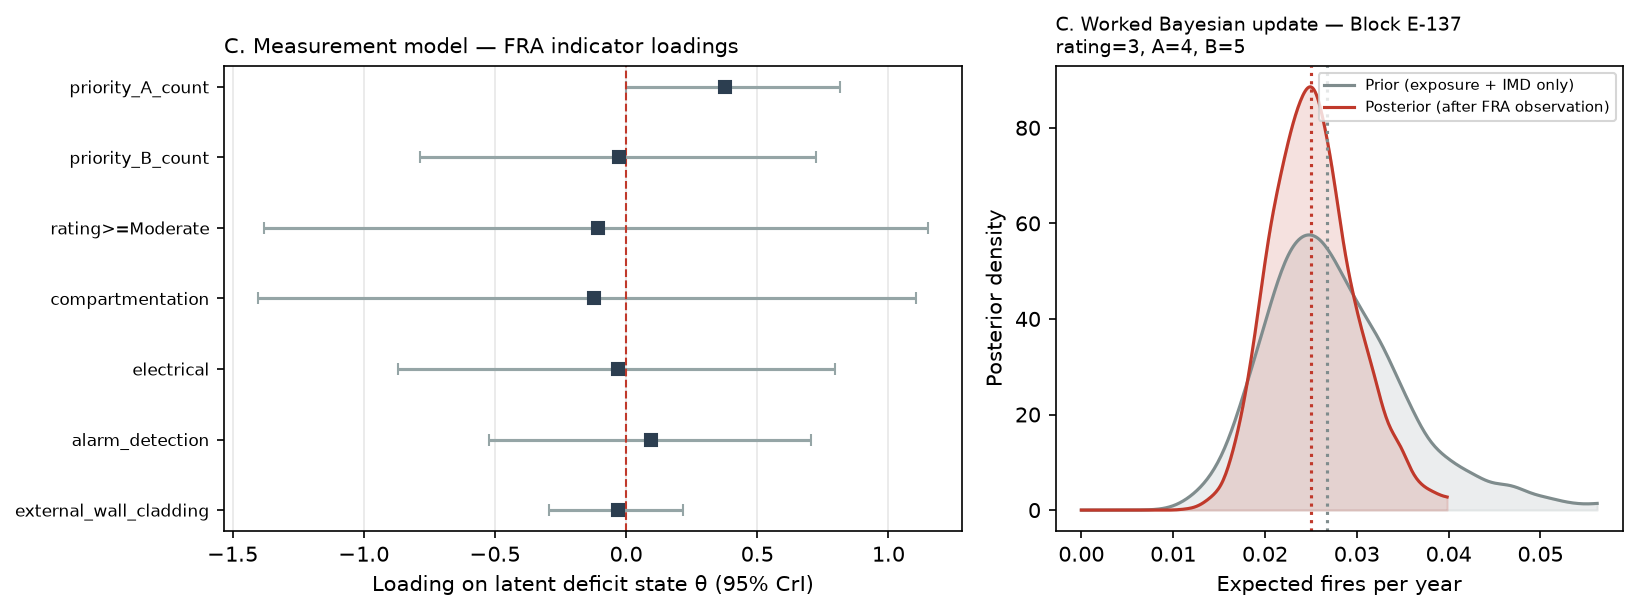
\includegraphics[width=0.9\linewidth]{figures/latent_worked_update.png}
  \caption{Worked single-block posterior update: conditioning on one estate's FRA
  observation shifts the expected fire-rate prior (95\% CrI 0.016--0.048 fires/year)
  to a tighter posterior (0.017--0.036). The inspection narrows the distribution ---
  the inspection-as-noisy-observation mechanism made numeric.}
  \label{fig:latent}
\end{figure}

\subsection{Ignition-source trends}
\label{sec:results-ignition}

Finally, a descriptive analysis of ignition sources over FY 2010/11--2024/25
(446{,}470 fires, Suffolk excluded from \emph{every} year to hold the 42-service
panel constant) fits a per-level generalised linear model (GLM) on fiscal year,
reporting each source's trend in its \emph{share} of dwelling fires
(Table~\ref{tab:ignition}, Figure~\ref{fig:ignition}). The clearest structural shift
is a broad, uniform decline in cooking-related ignition --- food as the ignited item
falls 10.8 percentage points, the single largest mover, alongside grills, hobs, ovens
and chip-pan fires --- consistent with safer appliance design. Against that backdrop
the fastest-rising identifiable source is the battery/electrical-apparatus family:
``battery charger'' fires rose $+425\%$ and ``apparatus --- batteries, generators''
$+86.8\%$, their combined share nearly tripling (1.28\% to 3.78\%, share odds ratio
1.059 per year).

The most useful finding, though, is a \emph{data-gap} one. The national taxonomy
cannot isolate the hazard the sector most fears: lithium-ion e-bike and e-scooter
fires have no dedicated category, and the only proxy (``batteries, generators'' plus
``battery charger'') nets device batteries with standby generators and predates the
e-mobility boom. London Fire Brigade's device-specific counts rose roughly thirtyfold
over 2017--2025 while the national proxy grew only about 72\% over fifteen years --- a
shape mismatch implying e-mobility fires are being absorbed into generic levels. We
flag this to MHCLG: a dedicated device-type sub-field is needed before the national
data can track this hazard. Separately, the rising ``Unspecified''/``Other'' buckets
($+2.6$ and $+2.0$ percentage points) are themselves a recording-drift flag --- a
growing ``don't know'' share erodes the precision of every other category, the battery
proxy included.

\begin{table}[htbp]
  \centering
  \caption{Biggest movers in ignition-source \emph{share} of dwelling fires,
  FY 2010/11--2024/25 (share odds ratio per year from a binomial GLM). The battery
  family rises fastest among identifiable sources; cooking-related sources fall
  broadly.}
  \label{tab:ignition}
  \small
  \begin{tabular}{@{}lccl@{}}
    \toprule
    Ignition source & $\Delta$ share (pp) & Share OR/yr & Trend \\
    \midrule
    Battery charger                      & $+0.44$  & 1.125 & rising ($+425\%$ count) \\
    Apparatus: batteries, generators     & $+2.06$  & 1.052 & rising ($+86.8\%$) \\
    Combined battery proxy               & $+2.50$  & 1.059 & rising \\
    Grill / toaster                      & $-3.02$  & 0.956 & falling \\
    Cooker incl.\ oven                   & $-0.72$  & 0.993 & falling \\
    Food (item ignited)                  & $-10.78$ & ---   & falling (largest mover) \\
    \bottomrule
  \end{tabular}
\end{table}

\begin{figure}[htbp]
  \centering
  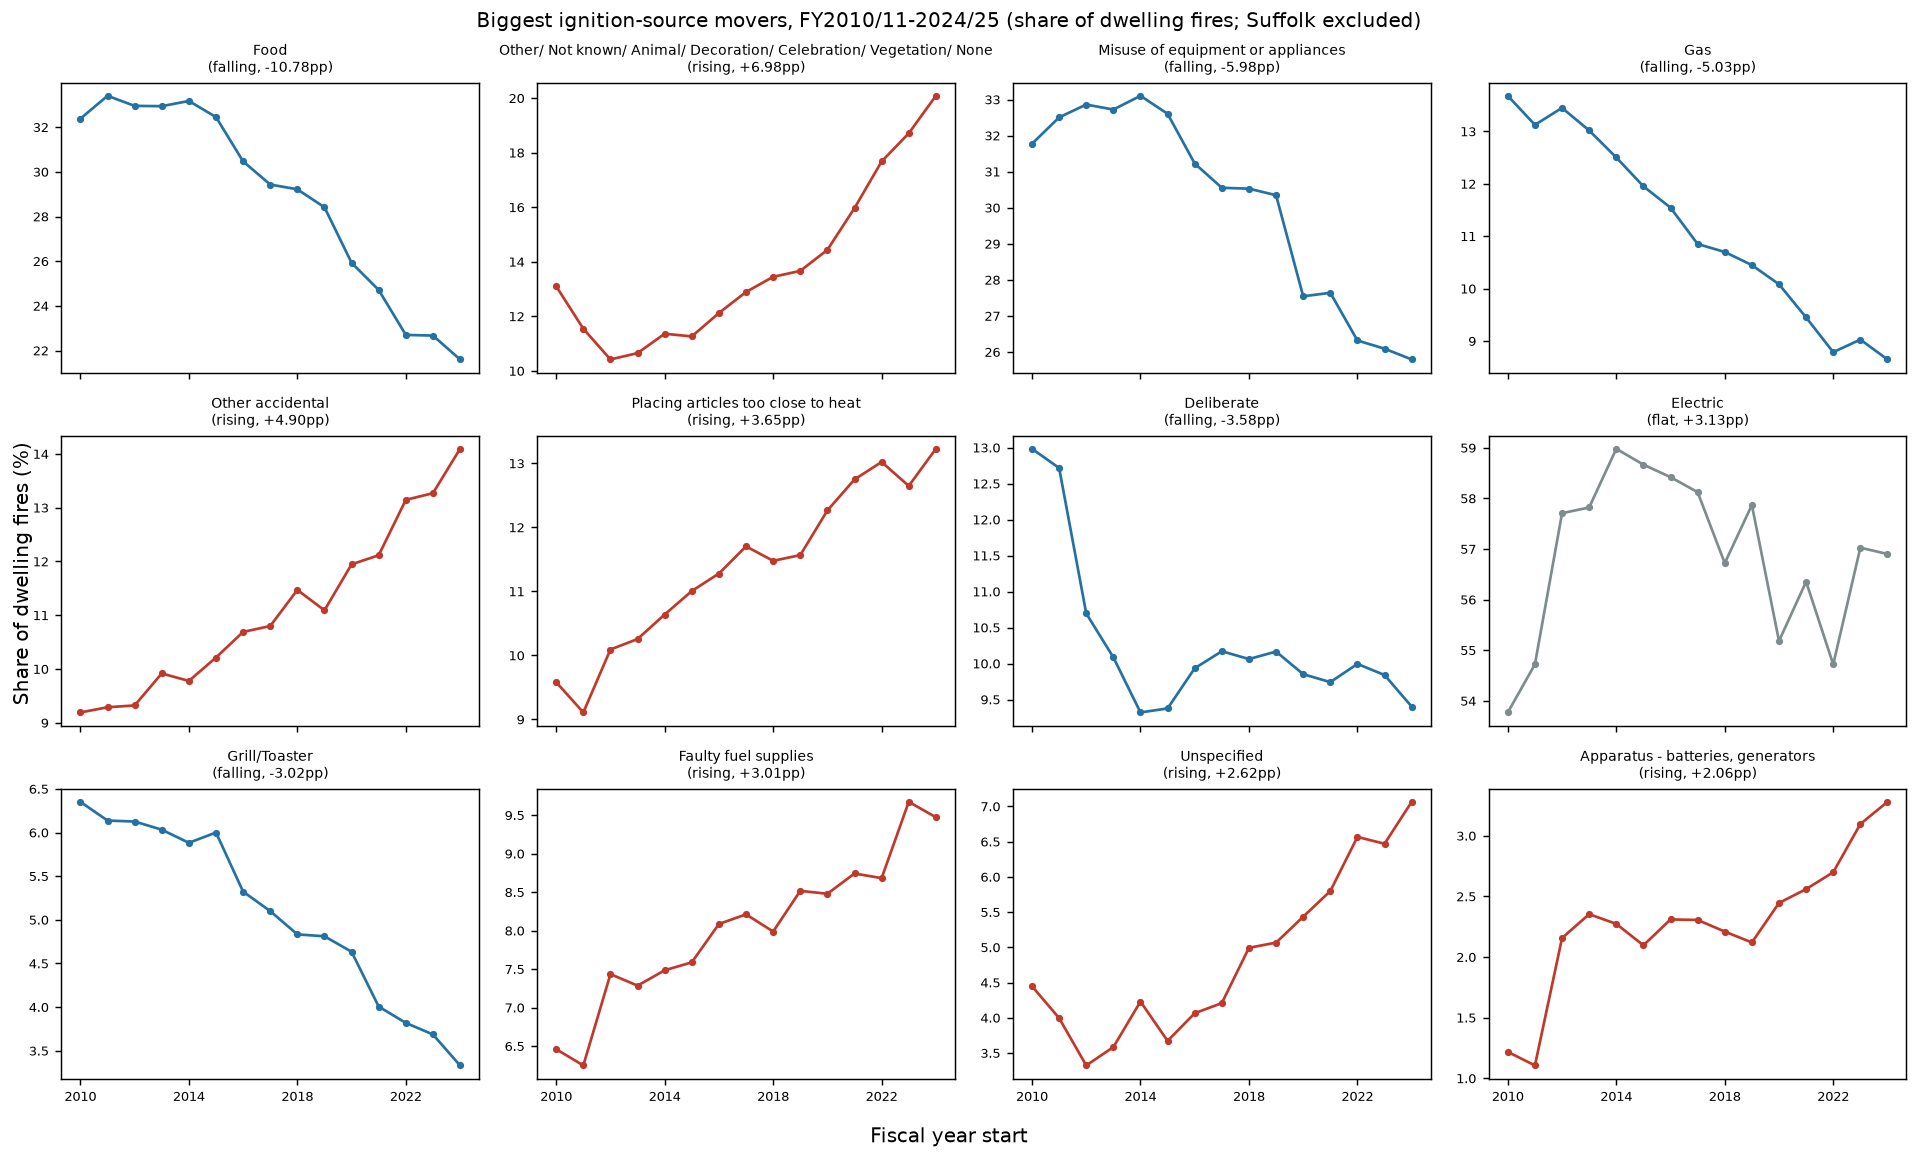
\includegraphics[width=0.82\linewidth]{figures/ign_small_multiples.png}
  \caption{Share trajectories of the twelve biggest-moving ignition sources, coloured
  by trend classification. Cooking sources decline broadly; the battery/apparatus
  family is the clearest riser after the generic ``Unspecified''/``Other'' buckets.}
  \label{fig:ignition}
\end{figure}

\section{Discussion and Limitations}
\label{sec:discussion}

The framework fits the post-Grenfell regulatory direction directly. Safety cases
under the Building Safety Act ask duty-holders to demonstrate that risks are
understood and managed on an ongoing basis \citep{grenfell2024phase2,bsa2022};
a posterior risk distribution with explicit credible intervals and
missing-evidence flags is a more faithful object for that purpose than a
categorical score, and the expected-value-of-inspection machinery turns the same
posterior into a prioritisation rule for where to spend finite inspection effort.
The results support the premise: the occurrence model is calibrated on held-out
years and recovers the deprivation gradient; the consequence models are calibrated
out-of-time and isolate a clean detection$\to$spread signal; and the simulator
reproduces the observed spread orderings while exposing an archetype-specific
mechanism (detection helps flats and houses, but not mobility-limited care homes)
that a purely statistical model would miss; and the value-of-targeting study puts a
conservative lower bound of a roughly ninefold return on that prioritisation over
untargeted allocation. Taken together they move FRA from a static compliance
checklist \citep{pas79_1_2020,pas79_2_2020} toward an updateable, evidence-based
risk picture --- with the fully sequential, inspection-assimilating version
specified in Section~\ref{sec:model} as the programme's next stage.

The real-building case study sharpens what the archetypes are for. Grounding the
high-rise-flat archetype against Grenfell Tower shows that its scale parameters ---
storeys and occupant load --- matter far less to modelled risk than its regime
assumptions: doubling the storeys shifts the exposed-household failure probability by
only 2\%, whereas losing compartmentation and abandoning stay-put shifts expected
fatalities by two orders of magnitude. The archetype is a sound geometric proxy
precisely because it already encodes the safety-critical single-stair topology; its
unavoidable simplification is that, like every archetype, it presumes the design
strategy holds. The same study marks the framework's outer boundary: an interior
room--corridor--stair graph cannot represent external cladding-driven spread, the
mechanism that drove Grenfell, and must defer to the external-wall and safety-case
regime of the Building Safety Act for that hazard. A real-geometry v2 pipeline ---
replacing archetype graphs with per-building layouts drawn from the downloadable
building-specification sources we catalogue (\texttt{docs/building\_specs\_sources.md})
--- is the natural next step, but the external-wall hazard will remain a regulated,
per-building duty rather than something a population-scale model should attempt.

Several limitations bound these claims, and we have kept them visible rather than
smoothing them over. This is an England-only residential MVP built on archetype
graphs, not real building geometry; the simulator is a transparent stochastic
caricature, not fire-physics CFD, and its multi-storey houses over-predict spread
beyond the floor of origin because of an idealised open internal stair; the
care-home archetype's building-level evacuation-failure rate overstates the
observed communal-living casualty rate by roughly $1.4\times$ per occupant ---
and far more ($\sim$$4.8\times$) at the building-level any-failure measure ---
reflecting its no-staff-assist, stay-put-free full-evacuation assumption. Both
headline posteriors are exact full-data objects --- the consequence models by
NUTS on all 451{,}172 records, the occurrence model by PSIS-corrected Laplace
importance sampling on all 202{,}530 training rows ($\hat{k}=0.33$;
Section~\ref{sec:model}) after full-data NUTS failed under three
parameterisations --- each corroborated by subsample NUTS, ADVI and MLE
cross-checks; the occurrence model's linear time trend under-predicts the
steeper 2024/25 decline. The consequence models are
covariate-adjusted associations, not causal effects: the casualty--alarm odds ratio
falls below one purely through occupancy confounding, which is precisely why the
model carries a latent-state layer, but that layer de-confounds by assumption and
structure rather than by identification, and this paper reports the adjusted
associations that feed it rather than a validated causal estimate. The FRS
response-time covariate carries little trustworthy independent signal: it is
ecological (identified at FRS$\times$year resolution and entangled with the secular
trend), and its effect on spread is not even robust in sign --- below one on the
subsample, above one at full data --- so we retain it only as a control and report no
directional response-time effect. The exact full-data fit exposes a further honest
gap: it undercovers per-service held-out counts (an FRS-overdispersion a single
random intercept misses), so per-service predictive intervals should be read as
anti-conservative and a random-slope extension is future work. Data linkage is imperfect --- record-level
fires resolve only to FRS area, not LSOA; covariates mix vintages (IMD 2025, Census
2021, EPC 2012--2026); and EPC attributes enter only as LSOA aggregates, consistent
with the address-level redistribution restriction of Section~\ref{sec:data}. Finally,
fire is a rare event, so building-level validation is not possible from open data: our
calibration is at the aggregate (LSOA-year and FRS-area) level, and the worked
building-level decomposition of Section~\ref{sec:results-synthesis} is illustrative of
the composition, not a validated per-building prediction.

\paragraph{Equity of targeted prevention.} Because fire risk is strongly
deprivation-linked, any risk-targeted allocation concentrates visits in deprived
areas. We regard this as the intended behaviour of a prevention programme ---
resources flow to where expected harm is greatest --- but it carries obligations
the framework should make explicit rather than bury in a score: targeting
criteria must be auditable (a virtue of interpretable rate ratios over black-box
scores), the uncertainty attached to any area's ranking should be visible to
decision-makers, and allocations should be monitored for unintended effects, such
as areas of genuinely high but poorly evidenced risk (wide posteriors) being
systematically deprioritised relative to areas that are merely well measured.
The expected-benefit policy of Section~\ref{sec:results-decision} partially
addresses the latter by valuing uncertainty reduction, but a full fairness
analysis of risk-targeted fire prevention --- who gains, who is overlooked, and
under which valuation of harm --- is future work we consider necessary before
operational deployment.

\paragraph{The physics programme.} The simulator's mechanism-informed status is a
staging point, not an endpoint. A companion work builds the corresponding physics
engine (NIST CFAST zone models over the same archetypes, with era-derived boundary
materials and design fires keyed to the national ignition-source distribution) and
calibrates its parameters against the observed English spread margins with a
model-discrepancy term. Its headline is a caution this paper's framing anticipates:
the calibrated physics reproduces the aggregate spread surface, but aggregate
margins identify only one physical parameter (effective door-openness) --- the
remainder require \emph{timed}, scenario-resolved calibration targets, which is a
further argument for the record-level data access discussed above.

\paragraph{Secondary findings with policy implications.} Two supporting analyses
sharpen the operational picture. The no-alarm spread penalty is not uniform across
households --- it is roughly twice the pooled value for lone pensioners
(Section~\ref{sec:results-interactions}) --- giving the targeting layer a concrete,
data-backed reason to up-weight areas rich in that group beyond what their fire rate
alone implies, precisely where consequence decouples from occurrence, while the night
penalty is a whole-stock effect that warrants no dwelling-specific multiplier. And the
ignition-source analysis surfaces a data-infrastructure gap: England's central
incident taxonomy cannot isolate lithium-ion e-bike and e-scooter fires, the hazard
the sector is most anxious about, so the most actionable recommendation there is not a
model change but a taxonomy one (Section~\ref{sec:results-ignition}).

\paragraph{The inspection layer, meeting data.} The sharpest test of the paper's
central claim --- that an FRA is a noisy observation, not a risk score --- is the first
instantiation of the inspection layer on real assessments
(Section~\ref{sec:results-latent}): the apparatus runs end to end on 1{,}441 published
assessments and a single inspection demonstrably narrows a block's fire-rate posterior,
yet on one cross-sectional wave the latent's coupling to fire rate is a
remediation-confounded null, so a snapshot FRA is \emph{not} a validated proxy for
persistent fire propensity. That is exactly the situation the framework is designed for
--- inspections assimilated as noisy evidence under explicit uncertainty --- and it
names the missing ingredient: a second assessment wave to turn the retrospective check
into a prospective test and point-identify the assessor-noise parameters.

\section{Conclusion}
\label{sec:conclusion}

We have recast UK residential fire risk assessment as Bayesian inference: risk is a
posterior distribution over ignition, spread, evacuation failure, and consequence,
updateable as evidence arrives, rather than a categorical score. The instantiated
components stand on their own evidence: a small-area occurrence model whose 50\%
and 90\% intervals cover 50.5\% and 90.2\% of held-out outcomes across all
33{,}755 English LSOAs, with calibration holding within deprivation, geography, and
building-form subgroups; consequence models that separate predictive association
from intervention effect and expose, rather than inherit, the confounds of
observational fire data; a mechanism-informed simulator whose orderings match the
national record and whose boundary a real-building stress test locates precisely;
and a decision layer in which the same posteriors allocate a fixed prevention
budget to roughly nine times the value of untargeted allocation --- above
break-even outright at small, concentrated budgets. The proposed latent-state
layer is now partially real: its measurement model is fitted on 1{,}441 published
fire risk assessments, a single inspection demonstrably narrows a building's risk
posterior, and the first empirical bounds on assessor detection sensitivity exist,
with a recovered two-wave pilot showing directly that findings persist while the
documentation trail under-records them. The novelty remains the integration ---
no prior work couples these elements in one auditable pipeline --- but the
integration now carries evidence at every joint. What stands between this
framework and live, building-resolved safety intelligence is data, not method:
repeated assessment waves to point-identify assessor noise and intervention
effectiveness, fine incident geography to nationalise the demonstrated sub-area
targeting gains, and timed outcomes to push physics-calibrated consequences past
their identifiability ceiling --- each a concrete, named acquisition rather than
an open research question.


\appendix
\section{Reproducibility}
\label{app:repro}

Every numbered figure and table in this paper traces to a results artifact under
\texttt{results/}, which traces to a module under \texttt{src/} that reads the
project database. The end-to-end map, environment (\texttt{requirements.txt},
frozen versions; Python~3.12), and the one-command database rebuild
(\texttt{python -m src.build\_db --with-epc --with-lfb}, or attach the shipped
DuckDB files) are documented in \texttt{REPRODUCE.md} at the repository root.
Priors are exactly as stated in the model sections
(Sections~\ref{sec:model}--\ref{sec:surrogate}); all sampler settings
(draws, warmup, chains, subsample sizes) live in the cited modules and are echoed
into each \texttt{results/*/summary.md}. All Monte Carlo and MCMC runs use fixed
seeds, listed below. Tables~\ref{tab:repro-fig1} and~\ref{tab:repro-tab1} give the
per-figure and per-table provenance; where a figure was regenerated from a saved
CSV rather than a module entry point, that is stated.

\begin{table}[htbp]
  \centering
  \small
  \setlength{\tabcolsep}{4pt}
  \caption{Reproducing each numbered \emph{figure}. Commands are run from the
  repository root inside the virtual environment; seeds are the module-level
  \texttt{SEED} constants.}
  \label{tab:repro-fig1}
  \begin{tabular}{@{}p{1.5cm}p{4.4cm}p{4.0cm}p{4.3cm}@{}}
    \toprule
    Figure & Producing module / function & Input artifacts & Seed(s) \& config \\
    \midrule
    \ref{fig:occ-cal} & \texttt{src.models.evaluate\_occurrence}
      (\texttt{fig\_calibration}); via \texttt{run\_occurrence eval}
      & occurrence posterior (\texttt{results/occurrence/}); held-out FY2023/24
      & \texttt{SEED=20240705} \\
    \ref{fig:occ-decile} & \texttt{src.models.evaluate\_occurrence}
      (\texttt{decile\_gradient\_fig}) & occurrence posterior; IMD deciles
      & \texttt{SEED=20240705} \\
    \ref{fig:cons-cal} & \texttt{src.models.consequence} (\texttt{fig\_reliability});
      regenerated from the out-of-time prediction CSV, not a standalone entry point
      & \texttt{results/consequence/} spread predictions
      & \texttt{SEED=20260705} \\
    \ref{fig:int-ame} & \texttt{src.models.interactions} (\texttt{fig\_ame\_heatmap})
      & \texttt{dwelling\_fires} (DB); alarm$\times$occupancy design
      & \texttt{SEED=20260705}; NUTS $4\times(800{+}1000)$ \\
    \ref{fig:sim-fail} & \texttt{src.sim.make\_report}
      (\texttt{fig\_failure\_by\_archetype}) & \texttt{results/sim/mc\_summary.csv}
      & sim \texttt{BASE\_SEED=20260705} \\
    \ref{fig:morris} & \texttt{python -m src.sim.morris\_sweep}
      & \texttt{results/sim/morris\_ee.csv}, \texttt{morris\_ranking.csv}
      & \texttt{BASE\_SEED=20260713}; 20 trajectories, 6 levels, 4{,}000 runs/cell \\
    \ref{fig:decision-sens} & \texttt{src.models.decision} (\texttt{fig\_sensitivity})
      & \texttt{results/} occurrence + consequence engines
      & \texttt{SEED=20260705} \\
    \ref{fig:london-targeting} & \texttt{src.models.london\_pilot}
      (\texttt{fig\_targeting}) & London 50\,m cell panel
      (\texttt{results/london\_pilot/}) & \texttt{SEED=20260706} \\
    \ref{fig:latent} & \texttt{src.models.latent\_state}
      (\texttt{figC\_measurement\_worked\_update}) & Camden FRA panel
      (\texttt{data/processed/fra/}) & \texttt{SEED=20260706} \\
    \ref{fig:ignition} & \texttt{src.models.ignition\_trends}
      (\texttt{small\_multiples\_movers}) & \texttt{dwelling\_fires} ignition-source
      shares & deterministic (no seed) \\
    \bottomrule
  \end{tabular}
\end{table}

\begin{table}[htbp]
  \centering
  \small
  \setlength{\tabcolsep}{4pt}
  \caption{Reproducing each numbered \emph{table}. Numbers are summarised into the
  named \texttt{results/*/summary.md} by the producing module.}
  \label{tab:repro-tab1}
  \begin{tabular}{@{}p{1.6cm}p{4.6cm}p{4.0cm}p{4.0cm}@{}}
    \toprule
    Table & Producing module / command & Input artifacts & Seed(s) \& config \\
    \midrule
    \ref{tab:datasets} & none --- hand-built from \texttt{data/sources/*.md}
      & public source catalogue & n/a (see \texttt{REPRODUCE.md} \S1) \\
    \ref{tab:occ-forest} & \texttt{python -m src.models.run\_occurrence fit}
      & occurrence posterior (\texttt{results/occurrence/summary.md})
      & \texttt{SEED=20240705}; exact full-data posterior via
      \texttt{python -m src.models.full\_is} (\texttt{SEED=20260714};
      unimodality probe \texttt{full\_is multistart} $\to$
      \texttt{fullis\_multistart.csv}) / \texttt{full\_exact} (\texttt{20260713}) \\
    \ref{tab:ablation} & \texttt{python -m src.models.spatial\_ablation fit}\,/\,\texttt{eval}
      & \texttt{results/occurrence/} (\texttt{ladder.log}, \texttt{\_v2})
      & \texttt{SEED=20240706} \\
    \ref{tab:alarm} & \texttt{python -m src.models.consequence}
      & \texttt{results/consequence/summary.md}
      & \texttt{SEED=20260705}; NUTS $4\times(800{+}1000)$ \\
    \ref{tab:proper} & \texttt{python -m src.models.consequence}
      & held-out proper scores (\texttt{results/consequence/})
      & \texttt{SEED=20260705}; NUTS $4\times(800{+}1000)$ \\
    \ref{tab:sim} & \texttt{python -m src.sim.run\_experiments --runs 10000}
      & \texttt{results/sim/mc\_summary.csv}
      & \texttt{BASE\_SEED=20260705} ($+101$ per cell), $N{=}10{,}000$ \\
    \ref{tab:decision} & \texttt{python -m src.models.decision}
      & \texttt{results/decision/summary.md}
      & \texttt{SEED=20260705} \\
    \ref{tab:budget} & \texttt{python -m src.models.decision}
      (\texttt{fig\_budget\_sweep} companion) & \texttt{results/decision/}
      & \texttt{SEED=20260705} \\
    \ref{tab:grenfell-assumptions} & \texttt{python -m src.sim.case\_study}
      & \texttt{results/case\_study/summary.md} & \texttt{BASE\_SEED=20260705} \\
    \ref{tab:casestudy} & \texttt{python -m src.sim.case\_study} \&\
      \texttt{src.sim.hindcast} & \texttt{results/case\_study/}
      & \texttt{BASE\_SEED=20260705} \\
    \ref{tab:bounds} & \texttt{python src/models/latent\_state.py run}
      & \texttt{results/latent\_state/summary.md} & \texttt{SEED=20260706} \\
    \ref{tab:ignition} & \texttt{python -m src.models.ignition\_trends}
      & \texttt{results/ignition\_trends/summary.md} & deterministic (no seed) \\
    \bottomrule
  \end{tabular}
\end{table}


{\footnotesize
\setlength{\columnsep}{18pt}
\begin{multicols}{2}
\bibliographystyle{plainnat}
\bibliography{references}
\end{multicols}
}

\end{document}
